\chapter{品質試験のデモンストレーション} \label{chap:demo}
品質試験項目のデモンストレーションを行った。
今回のデモンストレーションでは、品質試験項目として読み出し試験を行い、データベース機能や試験の流れを確認した。
この章の前半では開発したツールと試験で使用するソフトウェア、ハードウェアについて説明し、後にデモンストレーションの内容、各ソフトウェアの機能確認について述べる。

\section{デモンストレーションと機能確認}
上述したピクセル解析ツールを含む読み出し試験用ソフトウェアの機能確認を目的として、生産時における流れのデモンストレーションを行なった。
その詳細について以下に示す。

\subsection{用いたソフトウェア}

試験で用いたソフトウェアをいかに示す。
また、これらソフトウェアの概要を図\ref{readout_SW_overview}に示す。
\begin{itemize}
  \item YARR(commit:6b3ffe92)
  \item MongoDB(version: v4.2.6)
  \item ローカルDBウェブアプリケーション(tag: ldbtoolv1.4)
  \item 中央データベースとの同期ツール(tag: ldbtoolv1.4)
  \item ピクセル解析ツール(tag: v1.0.2)
  \item 時系列データ用データベース(InfluxDB\cite{5-6}(version: 1.8.0))
    \begin{itemize}
      \item 時系列情報に特化したデータベース。このシステムにおいては温度、電圧などDCS情報を時間情報と共に保存、管理するために用いる。
    \end{itemize}
  \item InfluxDB解析ソフト(Grafana\cite{5-7}(version: 5.1.0))
    \begin{itemize}
      \item InfluxDBに保存された情報の解析、閲覧に用いる。ウェブブラウザー上でDCSデータを閲覧することができる。
    \end{itemize}
  \item 電源操作用ソフト
    \begin{itemize}
      \item 電源を遠隔で操作し、モジュールに電圧を供給する。また電圧、電流値を取得し、InfluxDBにアップロードする。CERNで開発されているPySerial\cite{5-8}(commit:0d14fcdb)を改良し作成した。
    \end{itemize}
  \item 温度読み出し用ソフト
    \begin{itemize}
      \item GPIO通信により取得できるADC値を取得、温度に変換しInfluxDBへアップロードする処理を作成したもの。RaspberryPi上に保存し、処理を実行。
    \end{itemize}
\end{itemize}

\begin{figure}[bpt]\centering
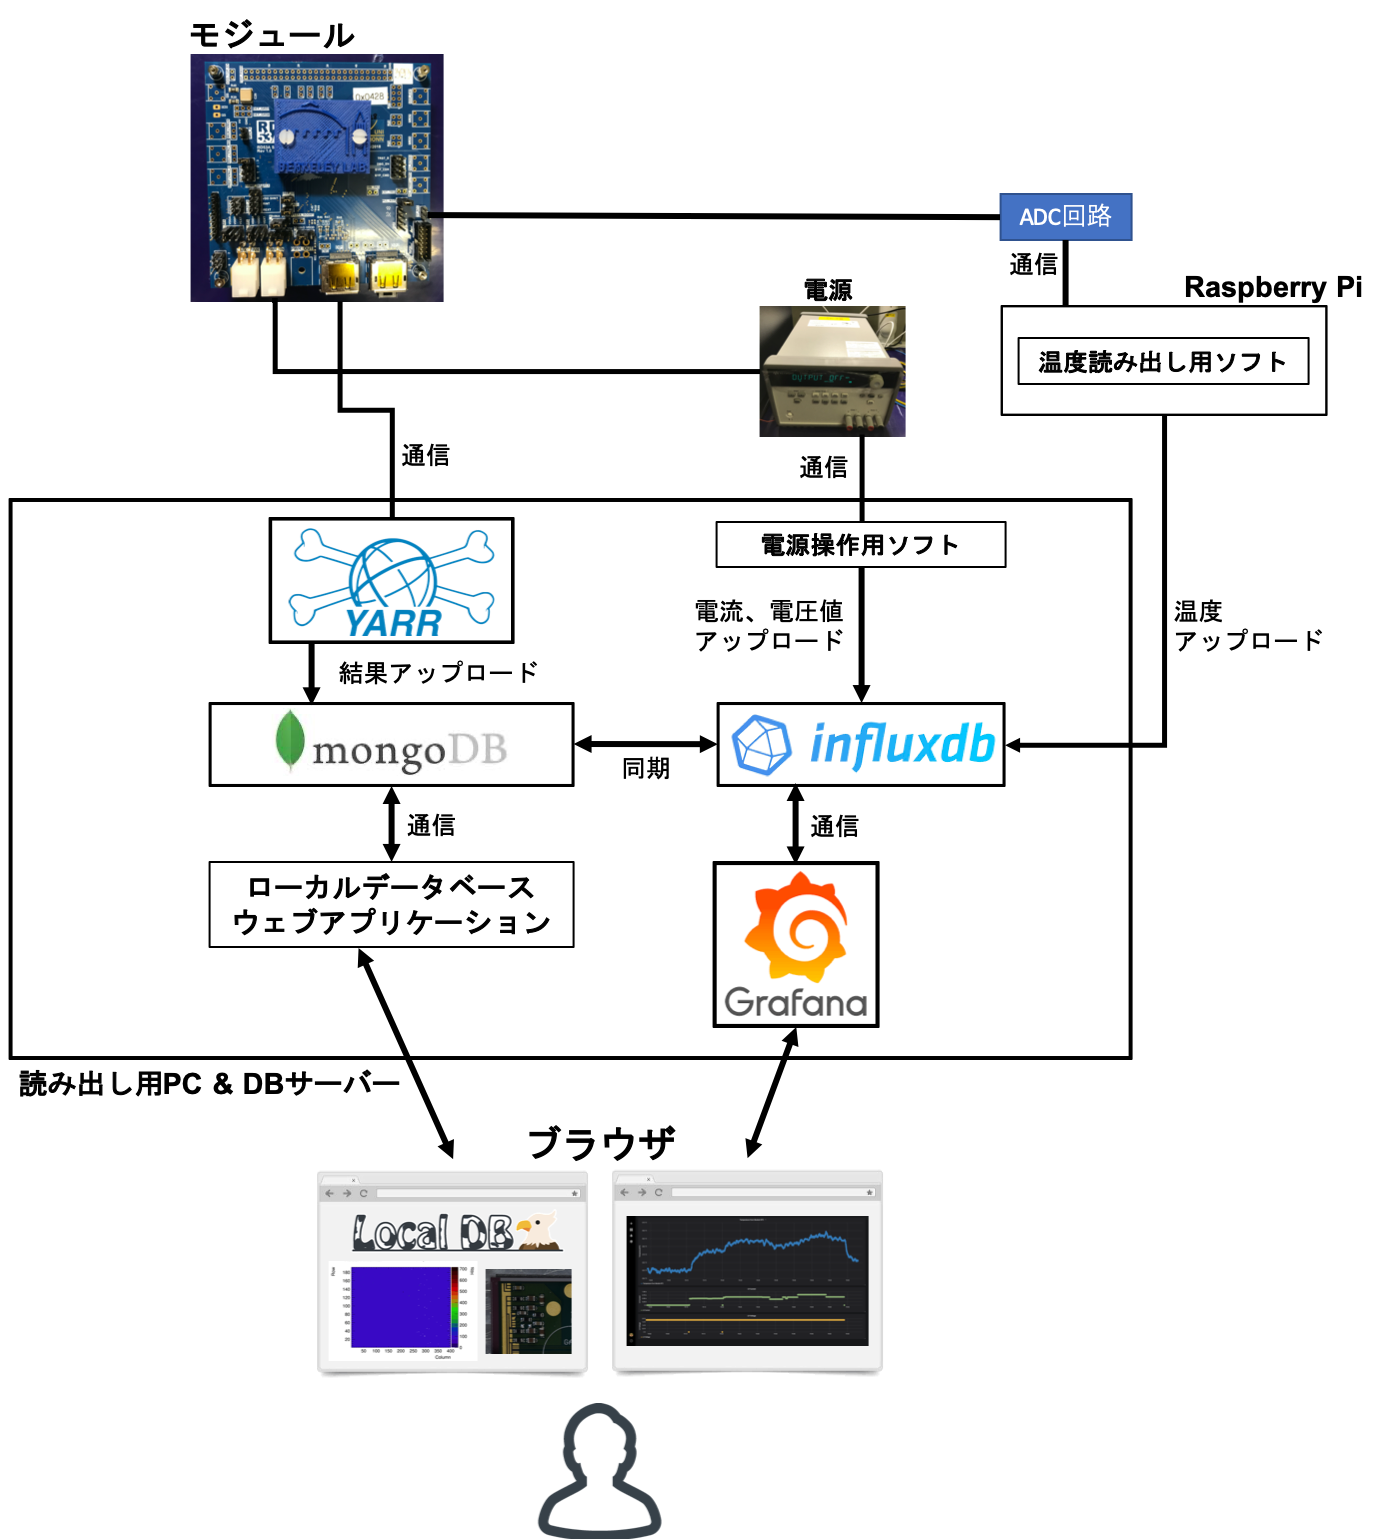
\includegraphics[width=14cm]{./readout_SW_overview.png}
\caption[読み出し試験に用いるソフトウェアの概要]{読み出し試験に用いるソフトウェアの概要。FEチップの読み出しとそのデータ通信はYARRを用いて行われる。試験結果はMongoDBにアップロードされ、試験者はウェブアプリケーションを通じて結果を確認することができる。電源操作用ソフトを用いて電源のスイッチ、電圧、電流値の取得がなされ、取得値はInfluxDBに保存される。モジュール付属のサーミスタ読み出しシステムを用いてFEチップ付近の温度を読み出し、InfluxDBに保存する。InfluxDBに保存されたDCSデータはGrafanaを用いてブラウザ上で確認することができる。またMongoDBに同期されるため、ローカルデータベースアプリケーションを通しても確認ができる。}
\label{readout_SW_overview}
\end{figure}

\clearpage
\subsection{用いたハードウェア}
読み出し試験に用いたハードウェアについて、以下に詳細を記す。

\subsubsection{RD53Aシングルモジュール(RD53A Single Chip Card, SCC)\cite{5-10}}
今回読み出しに使うモジュールとして、研究室で所有しているRD53Aシングルモジュール(RD53A Single Chip Card, SCC)を使用した。
SCCは試験用に作られたFEチップを一枚搭載するモジュールである。また今回使用したものはシリコンセンサーを持たない。
SCCはFEチップ電源端子、データ転送端子をもち、読み出しを行う際はそれぞれ配線をする。
FEチップ付近にはNTCサーミスタを搭載していて、ボード上の端子からその抵抗値を取得することで温度を測定することができる。
図\ref{demo_rd53a_SCC}に写真を示す。

\begin{figure}[h]\centering
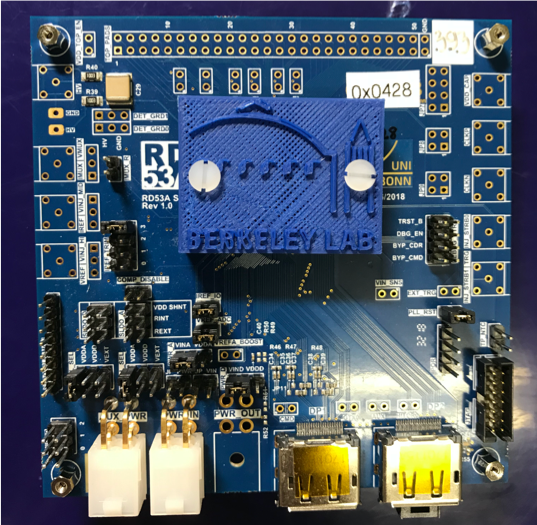
\includegraphics[width=7cm]{./rd53a_SCC.png}
\caption[RD53Aシングルモジュール(SCC)]{RD53Aシングルモジュール(SCC)\cite{5-10}。RD53AのFEチップを一枚搭載したモジュールである。図の中心部の青いカバーで囲われた中にFEチップが設置されている。このボード上にはデータ転送端子、電源端子、サーミスタ抵抗取得端子が設置されており、これらの端子に対応する配線をすることで読み出し試験のセットアップを組む。}
\label{demo_rd53a_SCC}
\end{figure}

\subsubsection{モジュールサーミスタ温度読み出しシステム}
モジュール付属サーミスタの抵抗値を取得し温度を測定するために、ADC、Raspberry Piを用いた温度読み出しシステムを作成した。
このシステムの中で扱った装置を表\ref{demo_temp_device}に、回路図、実際に配線した様子を図\ref{demo_temp_circit_pic}に示す。
スクリプト上でサーミスタの抵抗値に対応するADC値を温度に変換することで読み出しを行っている。
ADC値はGPIO通信\cite{5-9}により取得している。

\begin{table}[tbp]
\begin{center}
\caption[温度読み出しシステムに使用した装置一覧]{温度読み出しシステムに使用した装置一覧。}
\label{demo_temp_device}
  \small
  \begin{tabular}{|ll|} \hline
    装置 & 機種 \\ \hline
    10$\rm{k\Omega}$抵抗 & - \\
    ADC & MCP3002\cite{5-3} \\  
    RaspberryPi &  Raspberry Pi 3 Model B Plus Rev 1.3\cite{5-4} \\ \hline 
  \end{tabular}
\end{center}
\end{table}

\begin{figure}[h]\centering
  \begin{minipage}{0.5\hsize}
    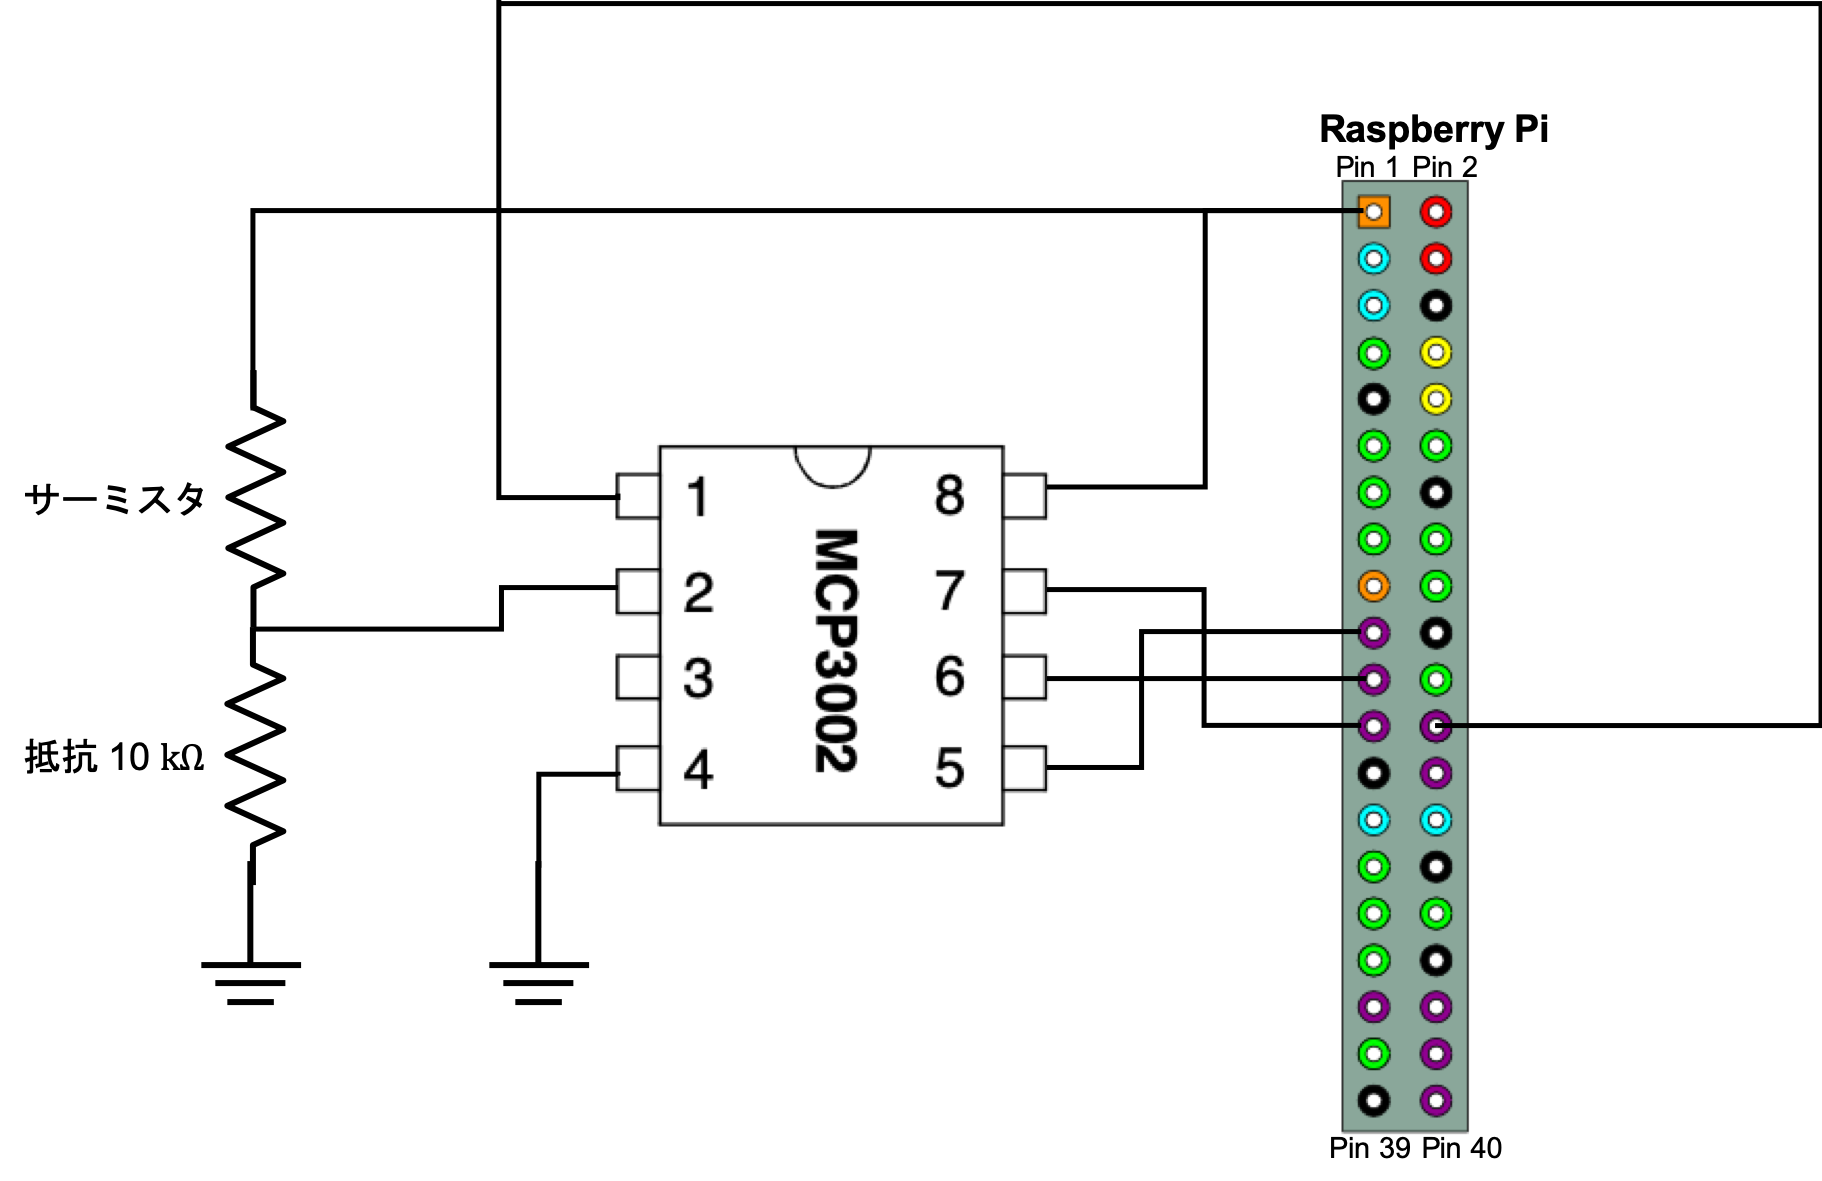
\includegraphics[width=6cm]{./temp_circit.png}
  \end{minipage}
  \begin{minipage}{0.4\hsize}
    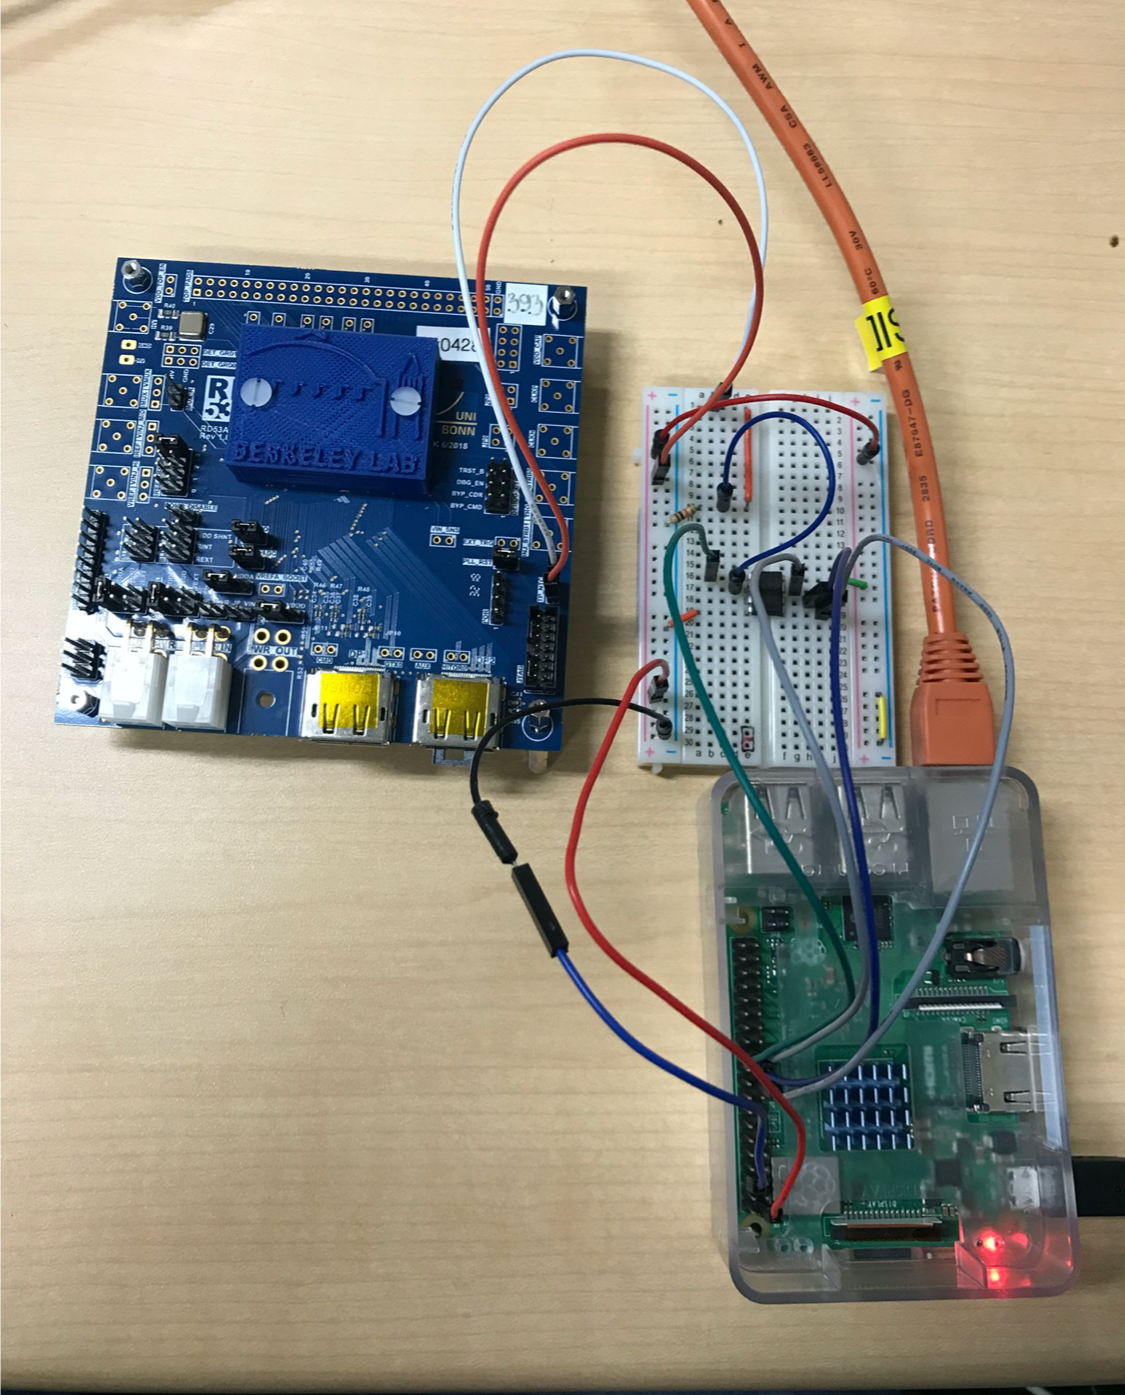
\includegraphics[width=4cm]{./temp_circit_pic.png}
  \end{minipage}
\caption[モジュール付属サーミスタを用いた温度読み出し回路]{モジュール付属サーミスタを用いた温度読み出し回路。図は回路図(左図)と実際に配線し、読み出しを行っている様子(右図)を示している。抵抗、MCP3002、Raspberry Piを用いて読み出し回路を作成した。抵抗とMCP3002は右図のようにブレッドボード上に設置した。ADCとRaspberryPiはGPIO通信\cite{5-9}を行うことで、ADC値を取得している。}
\label{demo_temp_circit_pic}
\end{figure}

\subsubsection{電源}
モジュールのFEチップに対する電圧供給にKEYSIGHTのE3646A 60Wデュアル出力電源\cite{5-1}(図\ref{demo_power_supply})を用いた。
\begin{figure}[h]\centering
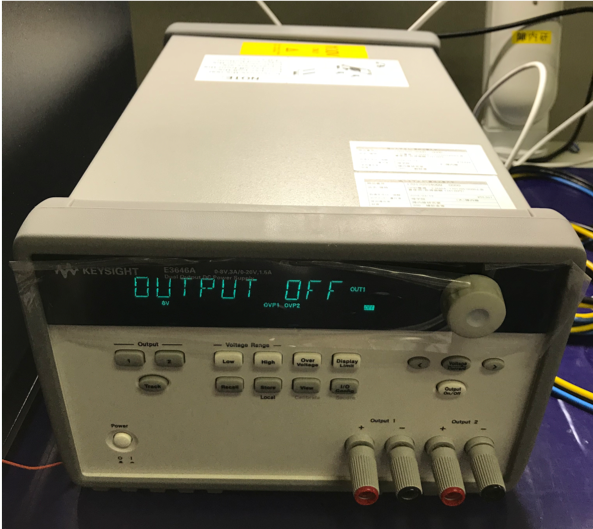
\includegraphics[width=5cm]{./power_supply.png}
\caption[用いた電源]{用いた電源。 FEチップ電圧供給のための電源としてKEYSIGHTのE3646A 60Wデュアル出力電源\cite{5-1}を用いた。}
\label{demo_power_supply}
\end{figure}

\subsubsection{FPGAボード}
FPGAボードにXpressK7\cite{5-2}を用いて、YARRファームウェアをFEGA上にプログラムし通信を行なった。
XpressK7を図\ref{demo_fpga_board}に示す。

\subsubsection{FMC-DisplayPort変換カード}
FPGAボードにはFMC端子がついていて、これをモジュールを接続するためにはFMC-DisplayPort変換カードが必要となる。
使用した変換カード(オハイオカード)を図\ref{demo_ohio}に示す。

\begin{figure}[htbp]
 \begin{minipage}{0.5\hsize}
  \begin{center}
   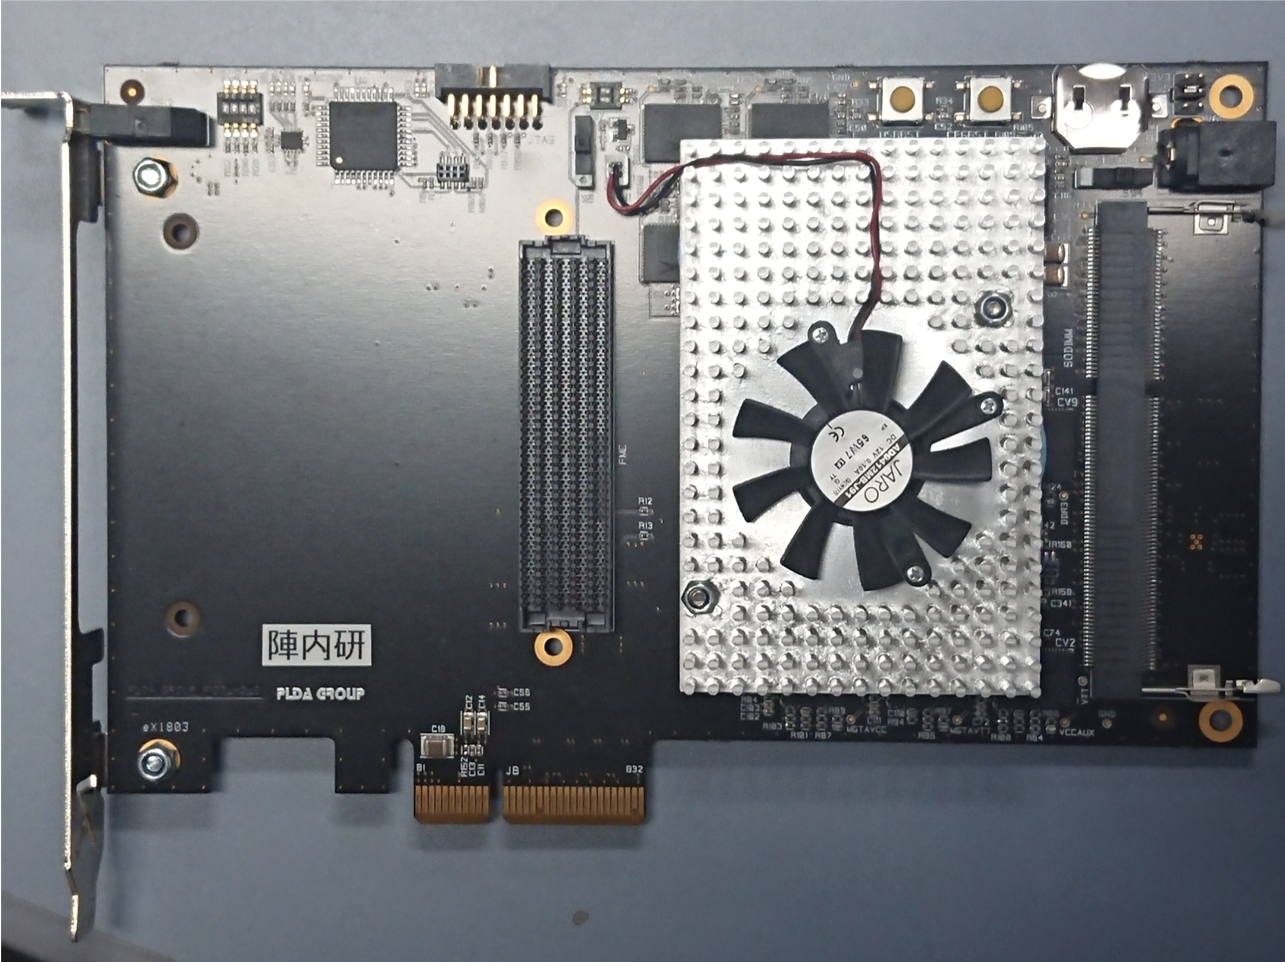
\includegraphics[width=50mm]{./fpga_board.png}
  \end{center}
  \caption[使用したFPGAボード(XpressK7)]{使用したFPGAボード(XpressK7\cite{5-2})。中央にFMC端子、右側にFPGAチップ、下側にPCI Expressが配置されている。FPGAチップの上にはファンをつけているため、この図では確認できない。}
  \label{demo_fpga_board}
 \end{minipage}
 \begin{minipage}{0.5\hsize}
  \begin{center}
   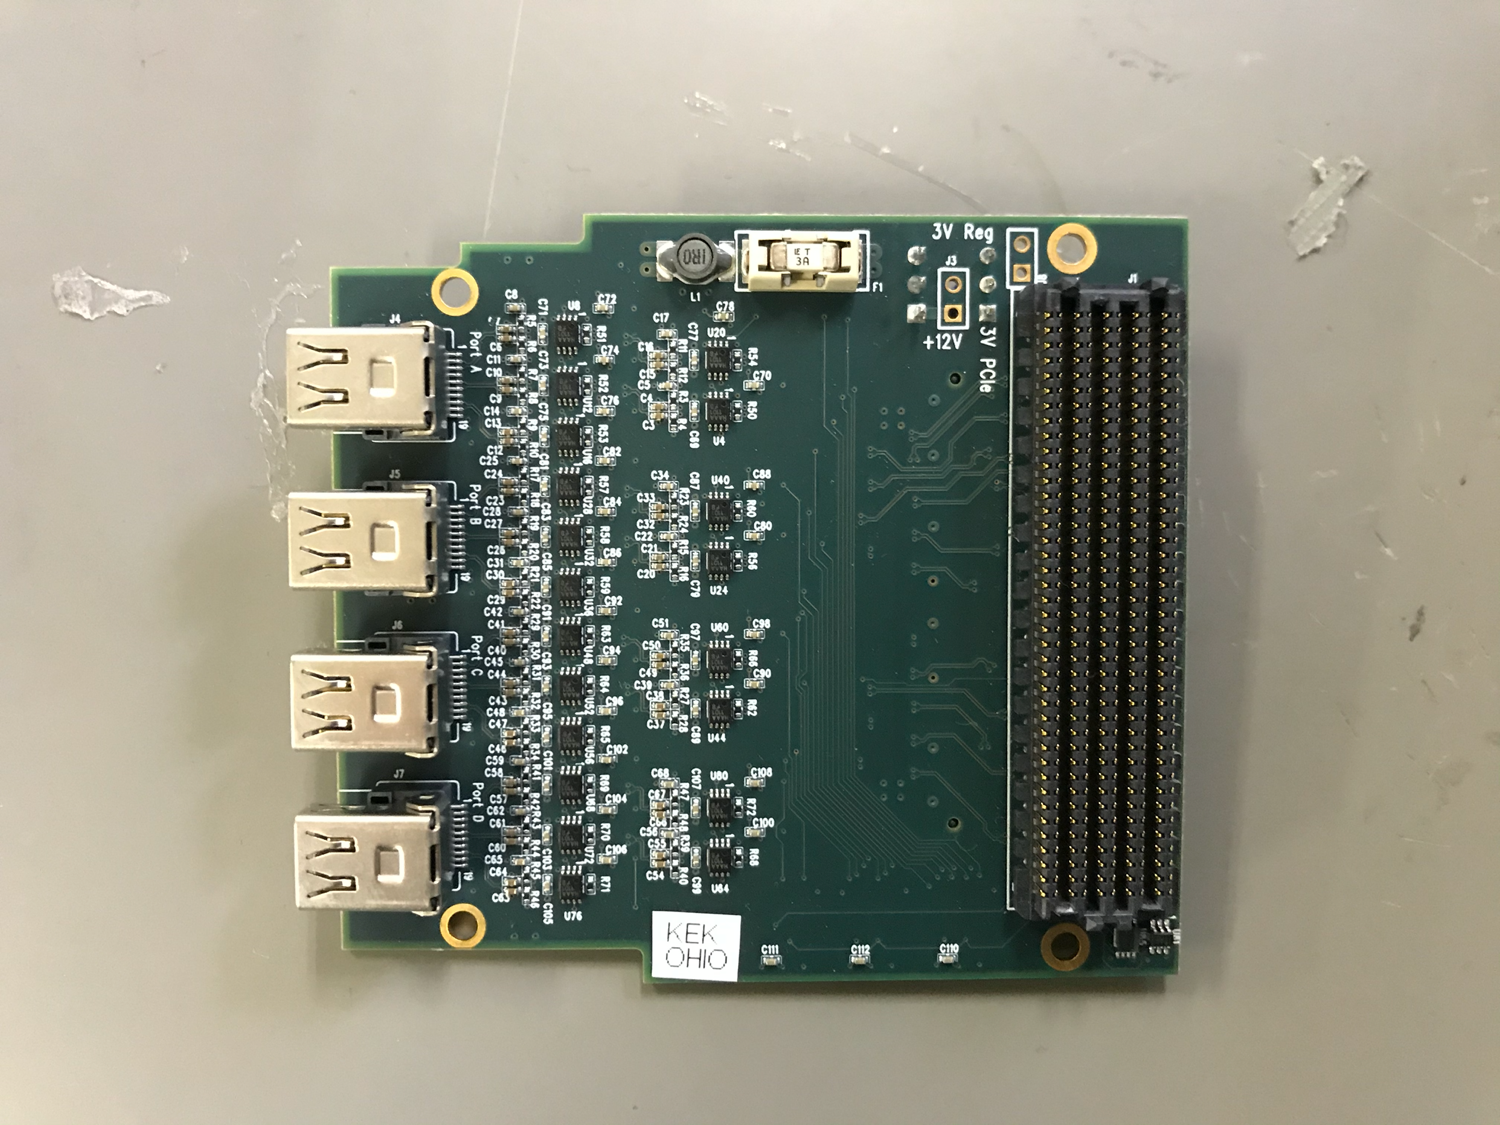
\includegraphics[width=50mm]{./ohio.png}
  \end{center}
  \caption[使用したFMC-DisplayPort変換カード(オハイオカード)]{使用したFMC-DisplayPort変換カード(オハイオカード)。図の右側にFMC端子、左側にminiDisplayPortが4つ配置されており、FMC端子を4つのminiDisplayPortに変換する。今回読み出すFEチップは1枚であるため、1つの端子だけを用いる。}
  \label{demo_ohio}
 \end{minipage}
\end{figure}

\subsubsection{PC}
YARRソフトウェアをインストールし、読み出しを行なったPCの性能を表\ref{daq_machine_spec}に示す。
\begin{table}[tbp]
\begin{center}
\caption[読み出しに使用したPCの性能]{読み出しに使用したPCの性能。研究室で所有するPCを使用した。OSはcentOS7である。}
\label{daq_machine_spec}
\scalebox{0.9}{
  \small
  \begin{tabular}{|llll|l|l|} \hline
    CPU & & & & Memory & Disk \\
    Type & Core & Thread & Clock speed[GHz]& [GB] & [GB] \\ \hline 
    Intel(R) Core(TM) i7-8700K CPU & 6 & 12 & 3.7 & 16.18 & 214\\ \hline
  \end{tabular}
}
\end{center}
\end{table}

\subsubsection{セットアップ}
読み出し試験に用いるハードウェアのセットアップを概要を図\ref{readout_setup_overview}に示す。

\begin{figure}[bpt]\centering
  \begin{minipage}{0.5\hsize}
    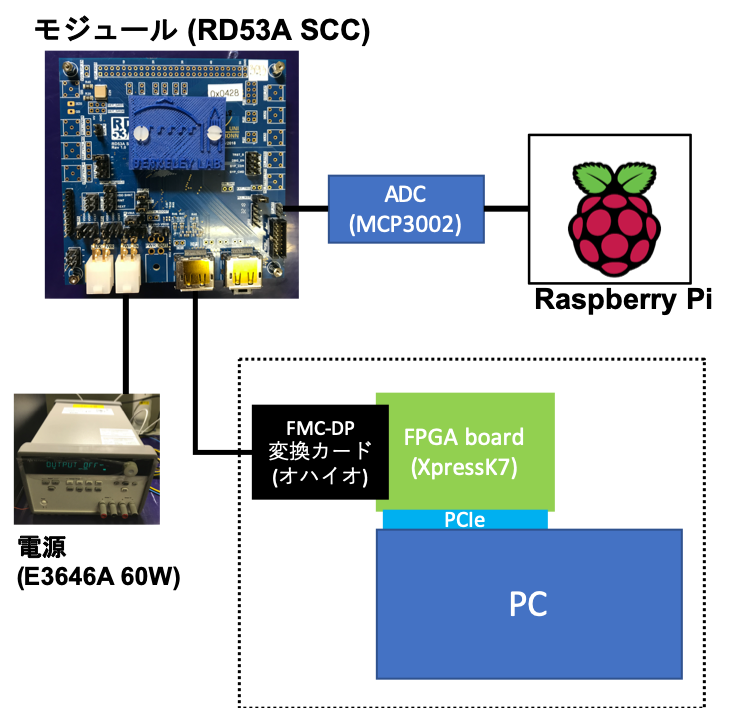
\includegraphics[width=6cm]{./HW_setup.png}
  \end{minipage}
  \begin{minipage}{0.4\hsize}
    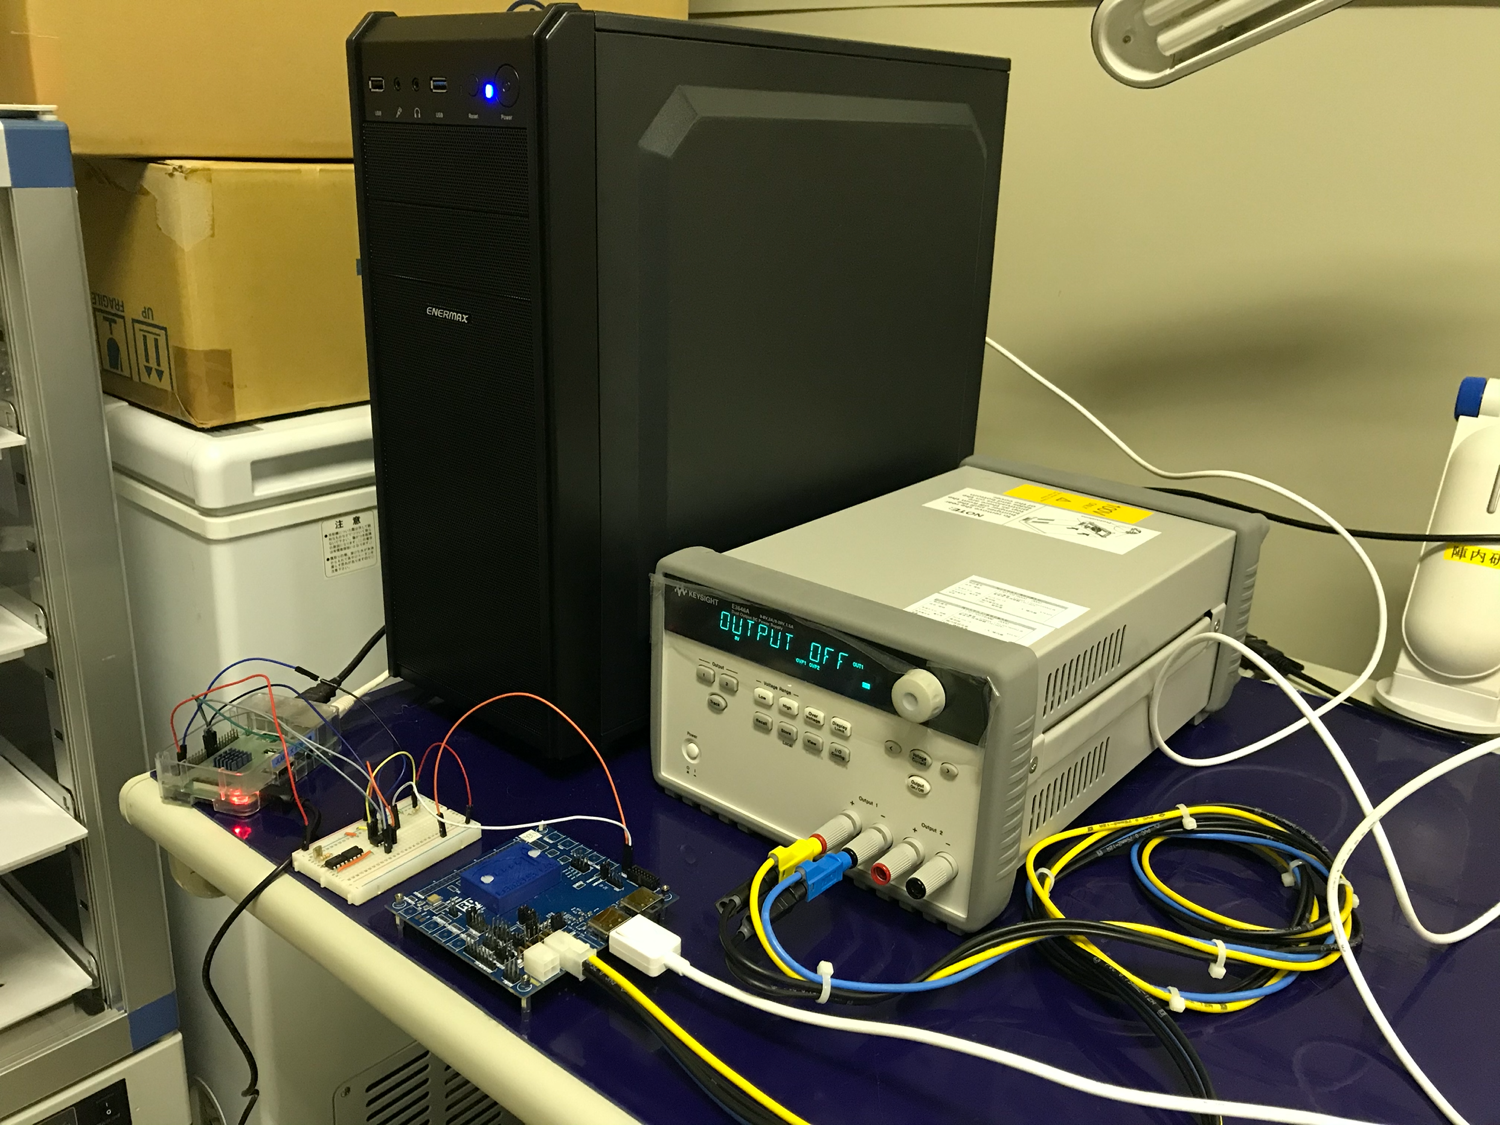
\includegraphics[width=5.5cm]{./HW_setup_pic.png}
  \end{minipage}
\caption[ハードウェアセットアップ]{ハードウェアセットアップ。図はセットアップの概要(左図)と実際に設置した様子(右図)を示している。FEチップ読み出し装置、電源、サーミスタ読み出し装置をそれぞれ設置、配線し、読み出し操作、データ取得を行った。}
\label{readout_setup_overview}
\end{figure}


%%%%%%%%%%%%%%%%%%%%%%%%%%%%%%%%%%%%%%%%%%%%%%%%%
%%%%%%%%%%%%%%%%%%%%%%%%%%%%%%%%%%%%%%%%%%%%%%%%%
%%%%%%%%%%%%%%%%%%%%%%%%%%%%%%%%%%%%%%%%%%%%%%%%%
\clearpage
\subsection{デモンストレーションの流れ}
デモンストレーションで用いるため、中央データベースにおける登録IDの定義方法\cite{5-11}に従い以下のモジュール、FEチップを登録した。

\begin{description}
  \item[モジュールID] 20UPGR00000001
  \item[FEチップID] 20UPGFC9999999
\end{description}
今回のデモンストレーションではこれらのIDを用いて試験結果の紐付け等のデータベース操作を行う。

確認した機能を行った流れの順に以下に示す。
\begin{enumerate}
  \item 中央データベースからモジュール情報のダウンロード.
  \item 読み出し試験実施、結果をローカルデータベースに保存.
  \item DCS情報の取得、監視.
  \item 試験結果検索.
  \item 試験結果閲覧.
  \item 結果選択とピクセル解析機能.
  \item 中央データベースへ試験結果のアップロード
\end{enumerate}

\subsection{機能確認}
読み出し試験を通して、各ソフトウェア機能が正しく動くことを確認した。
詳細を以下に記す。

\subsubsection{中央データベースからモジュール情報のダウンロード}
ダウンロードし、ウェブアプリケーションで確認した。
確認した画面を図\ref{demo_download_SCC}に示す。
今回行った試験結果はこのモジュールに紐つける形でローカルデータベースに保存される。

\begin{figure}[bpt]\centering
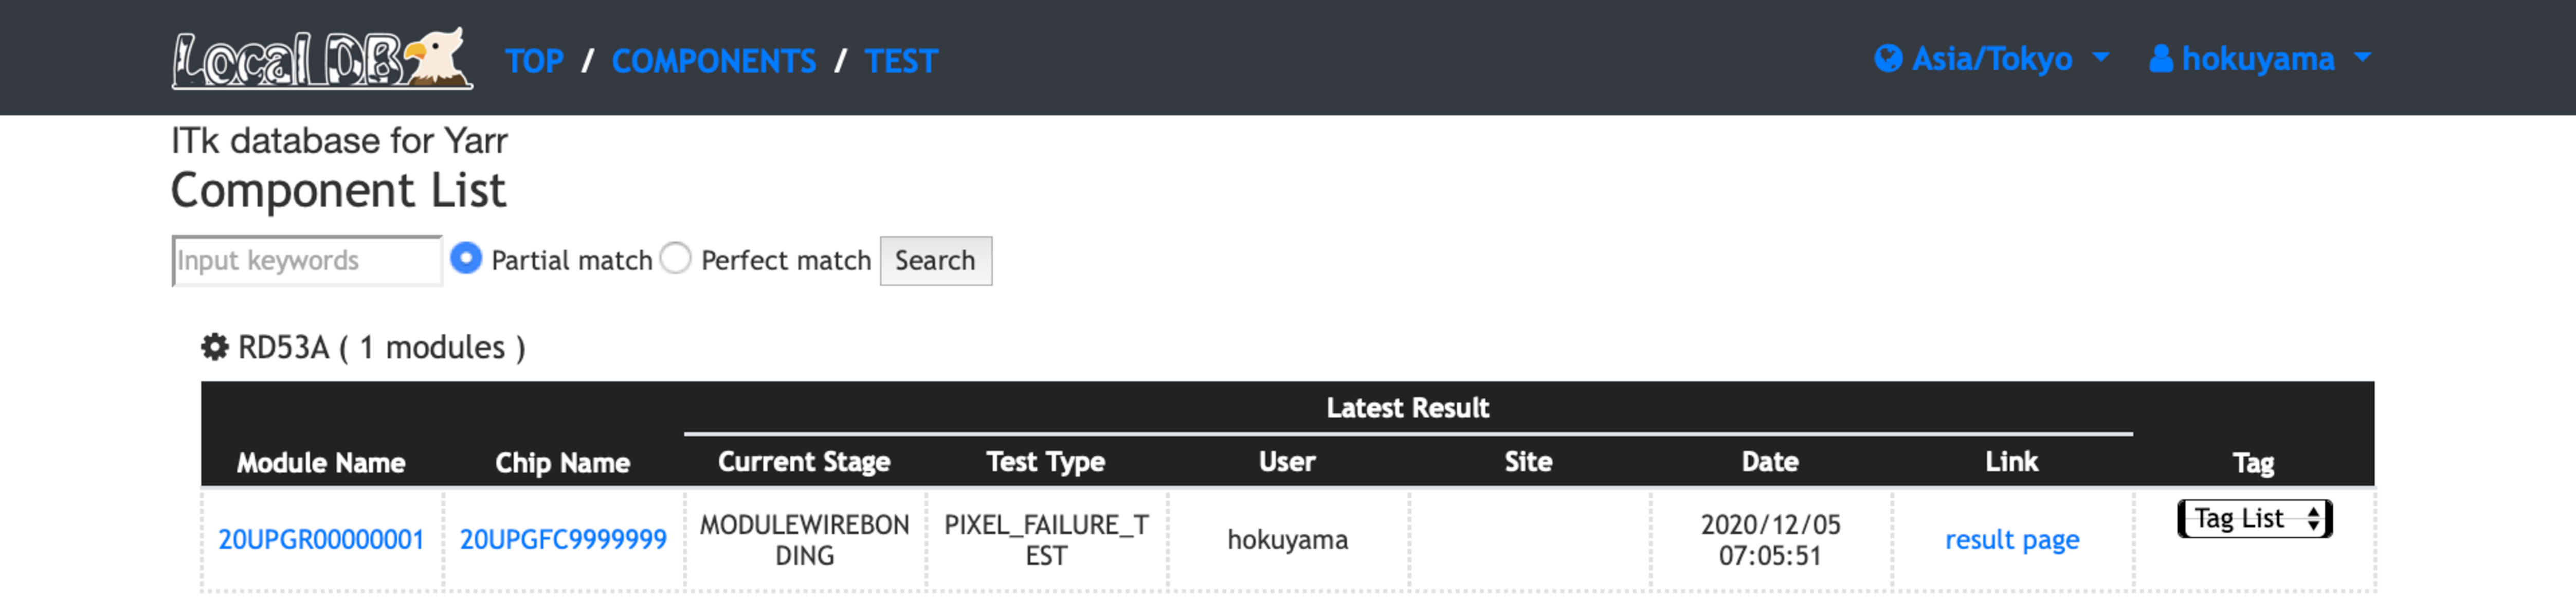
\includegraphics[width=16cm]{./demo_download_SCC.pdf}
\caption[ダウンロードしたモジュールID確認画面]{ダウンロードしたモジュールID確認画面。図の表において、今回登録した20UPGR00000001のIDを持つモジュールがローカルデータベースのウェブ上で確認できていることが分かる。また対応するFEチップのIDも確認することができる。}
\label{demo_download_SCC}
\end{figure}

%%%%%%%%%%%%%%%%%%%%%%%%%%%%%%%%%%%%%%%%%%%%%%%%%
%%%%%%%%%%%%%%%%%%%%%%%%%%%%%%%%%%%%%%%%%%%%%%%%%

\clearpage
\subsubsection{読み出し試験実施}
以下の流れに沿って読み出しを行ない、結果をローカルデータベースに保存した。
\begin{enumerate}
  \item デジタル回路読み出し(\texttt{std$\_$digitalscan})
  \item アナログ回路読み出し(\texttt{std$\_$analogscan})
  \item 調整前Threshold測定(\texttt{std$\_$thresholdscan})
  \item Threshold調整
  \item ToT調整
  \item Threshold再調整
  \item 調整後Threshold測定
  \item ToT測定(\texttt{std$\_$totscan})
  \item ノイズ測定(\texttt{std$\_$noisescan})
\end{enumerate}

また読み出し試験を通してDCS情報はInfluxDBを用いて監視し、試験結果と同様にローカルデータベースに保存した。

%%%%%%%%%%%%%%%%%%%%%%%%%%%%%%%%%%%%%%%%%%%%%%%%%
%%%%%%%%%%%%%%%%%%%%%%%%%%%%%%%%%%%%%%%%%%%%%%%%%
\subsubsection{DCS情報の監視}
読み出し試験は、DCS情報を監視しながら行った。
それぞれの値は対応するソフトウェアを用いてInfluxDBにアップロードした。
その値をGrafanaを使って監視をした。その様子を図\ref{demo_monitor_dcs}に示す。

\begin{figure}[bpt]\centering
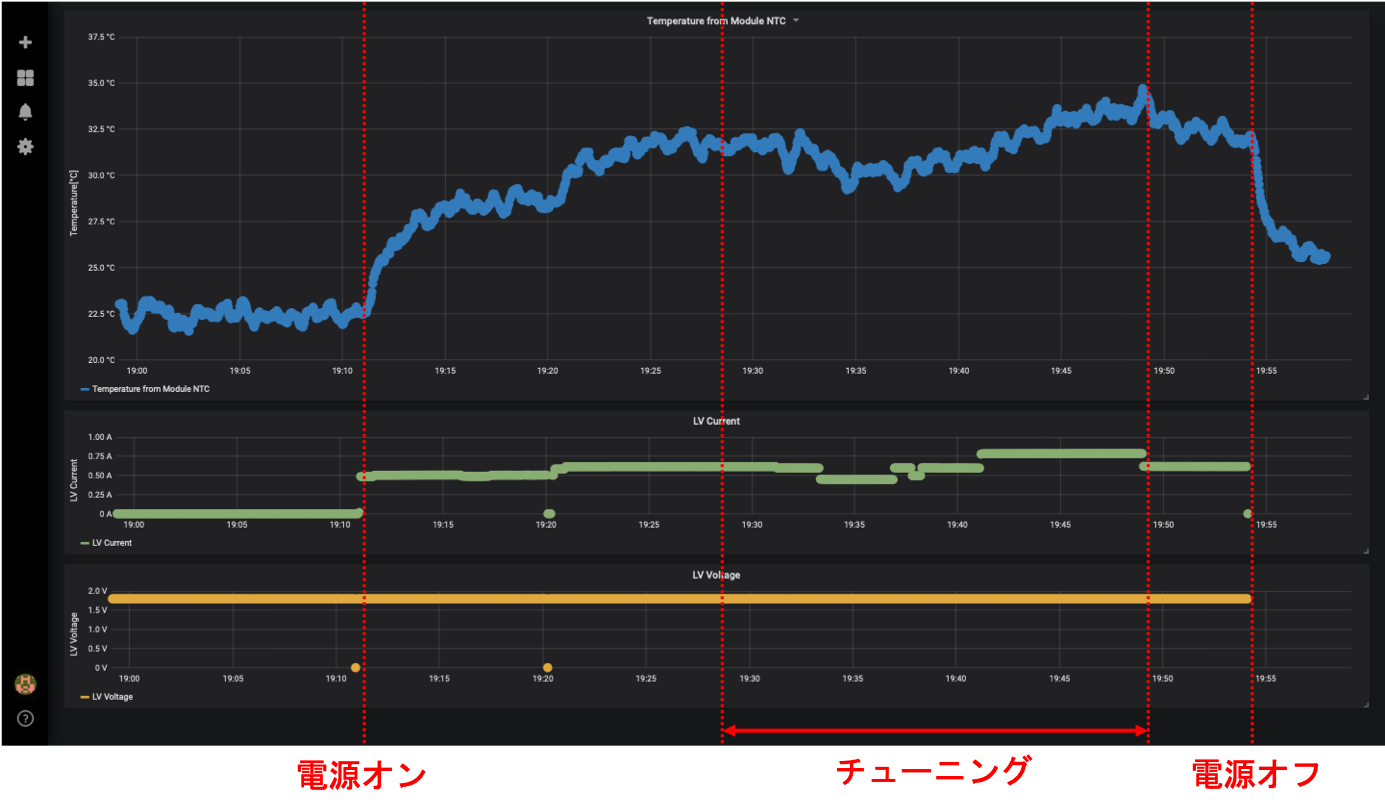
\includegraphics[width=15cm]{./demo_monitor_dcs.png}
\caption[DCS情報のモニタリングの様子]{DCS情報のモニタリングの様子。図において全て横軸は時間であり、縦軸は上から温度(青)、電流(緑)、電圧(黄)を示す。それぞれのデータの監視が行えていることが分かる。温度に関して、電源オン、オフの付近で変化が大きいことが分かる。電流に関して、読み出し(チューニング)を行っている途中にも微小変化していることが分かる。}
\label{demo_monitor_dcs}
\end{figure}

%%%%%%%%%%%%%%%%%%%%%%%%%%%%%%%%%%%%%%%%%%%%%%%%%
%%%%%%%%%%%%%%%%%%%%%%%%%%%%%%%%%%%%%%%%%%%%%%%%%
\clearpage
\subsubsection{検索機能}

検索機能の確認を行い、正常に使用できることを確認した。
検索機能実行の様子を図\ref{demo_search_function}に示す。

\begin{figure}[bpt]\centering
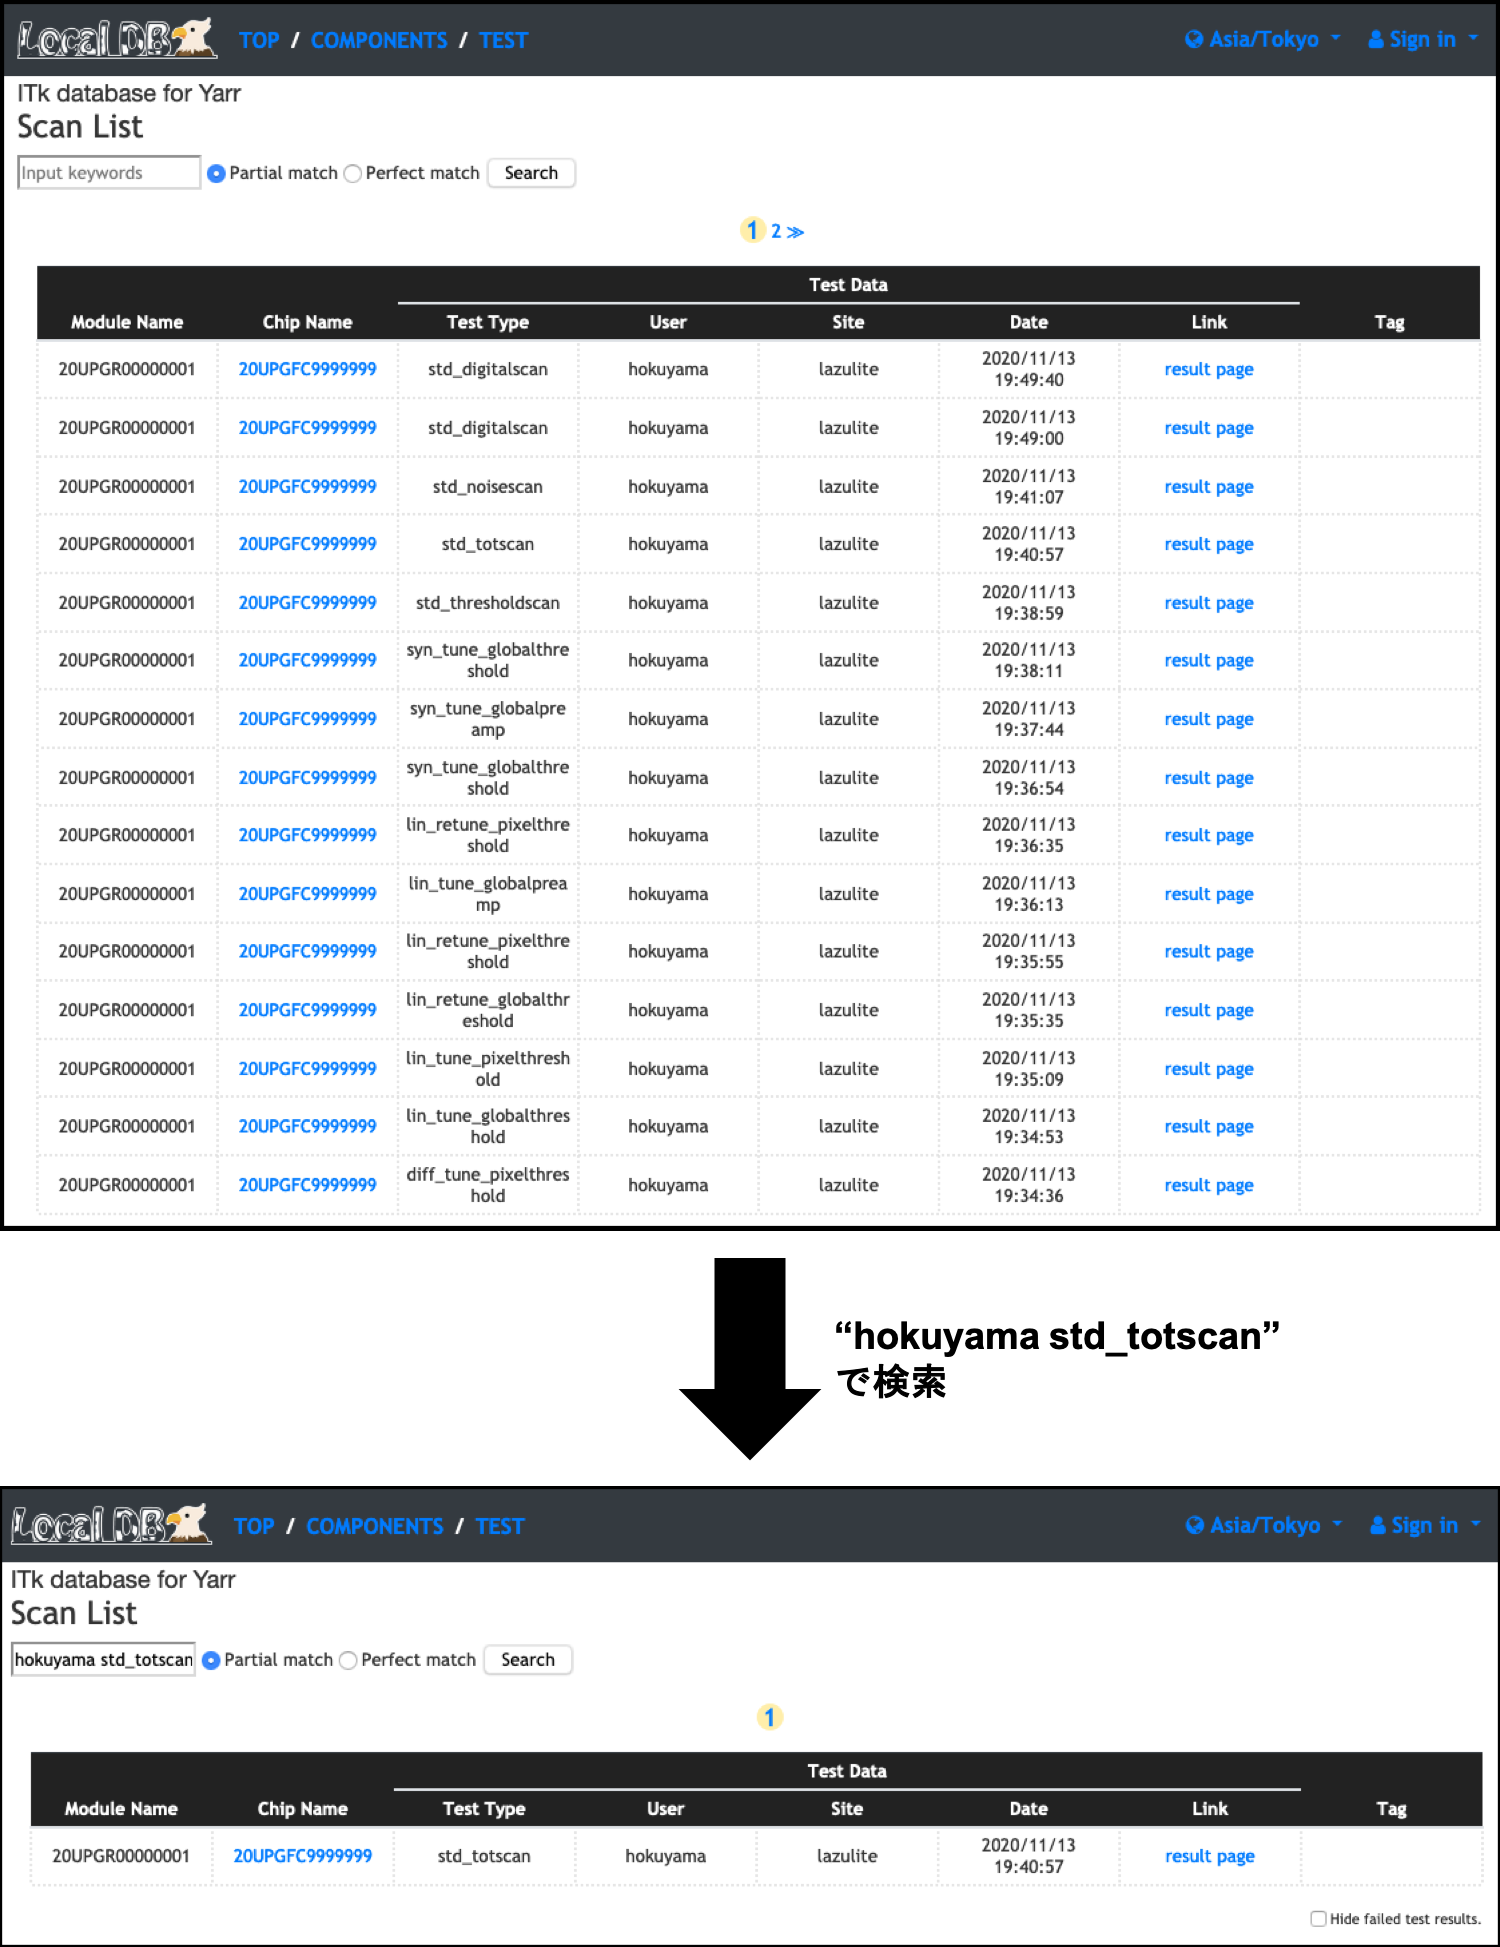
\includegraphics[width=13cm]{./demo_search_function.png}
\caption[検索機能確認の様子]{検索機能確認の様子。図は検索実行前の試験結果一覧(上図)と実行後(下図)を示す。図の例では"hokuyama std$\_$totscan"の2つのキーワードで検索を行っており、実行後は対応する試験結果1つが表示されていることが分かる。この試験結果について試験実施者は"hokuyama"、試験項目は"std$\_$totscan"であるため、検索機能が正常に動いていることが分かる。}
\label{demo_search_function}
\end{figure}

%%%%%%%%%%%%%%%%%%%%%%%%%%%%%%%%%%%%%%%%%%%%%%%%%
%%%%%%%%%%%%%%%%%%%%%%%%%%%%%%%%%%%%%%%%%%%%%%%%%
\clearpage
\subsubsection{試験結果閲覧}
ウェブアプリケーションを用いて、試験結果を閲覧した。その様子を図\ref{demo_view_result}に示す。
\begin{figure}[bpt]\centering
  \begin{minipage}{0.45\hsize}
    \begin{center}
    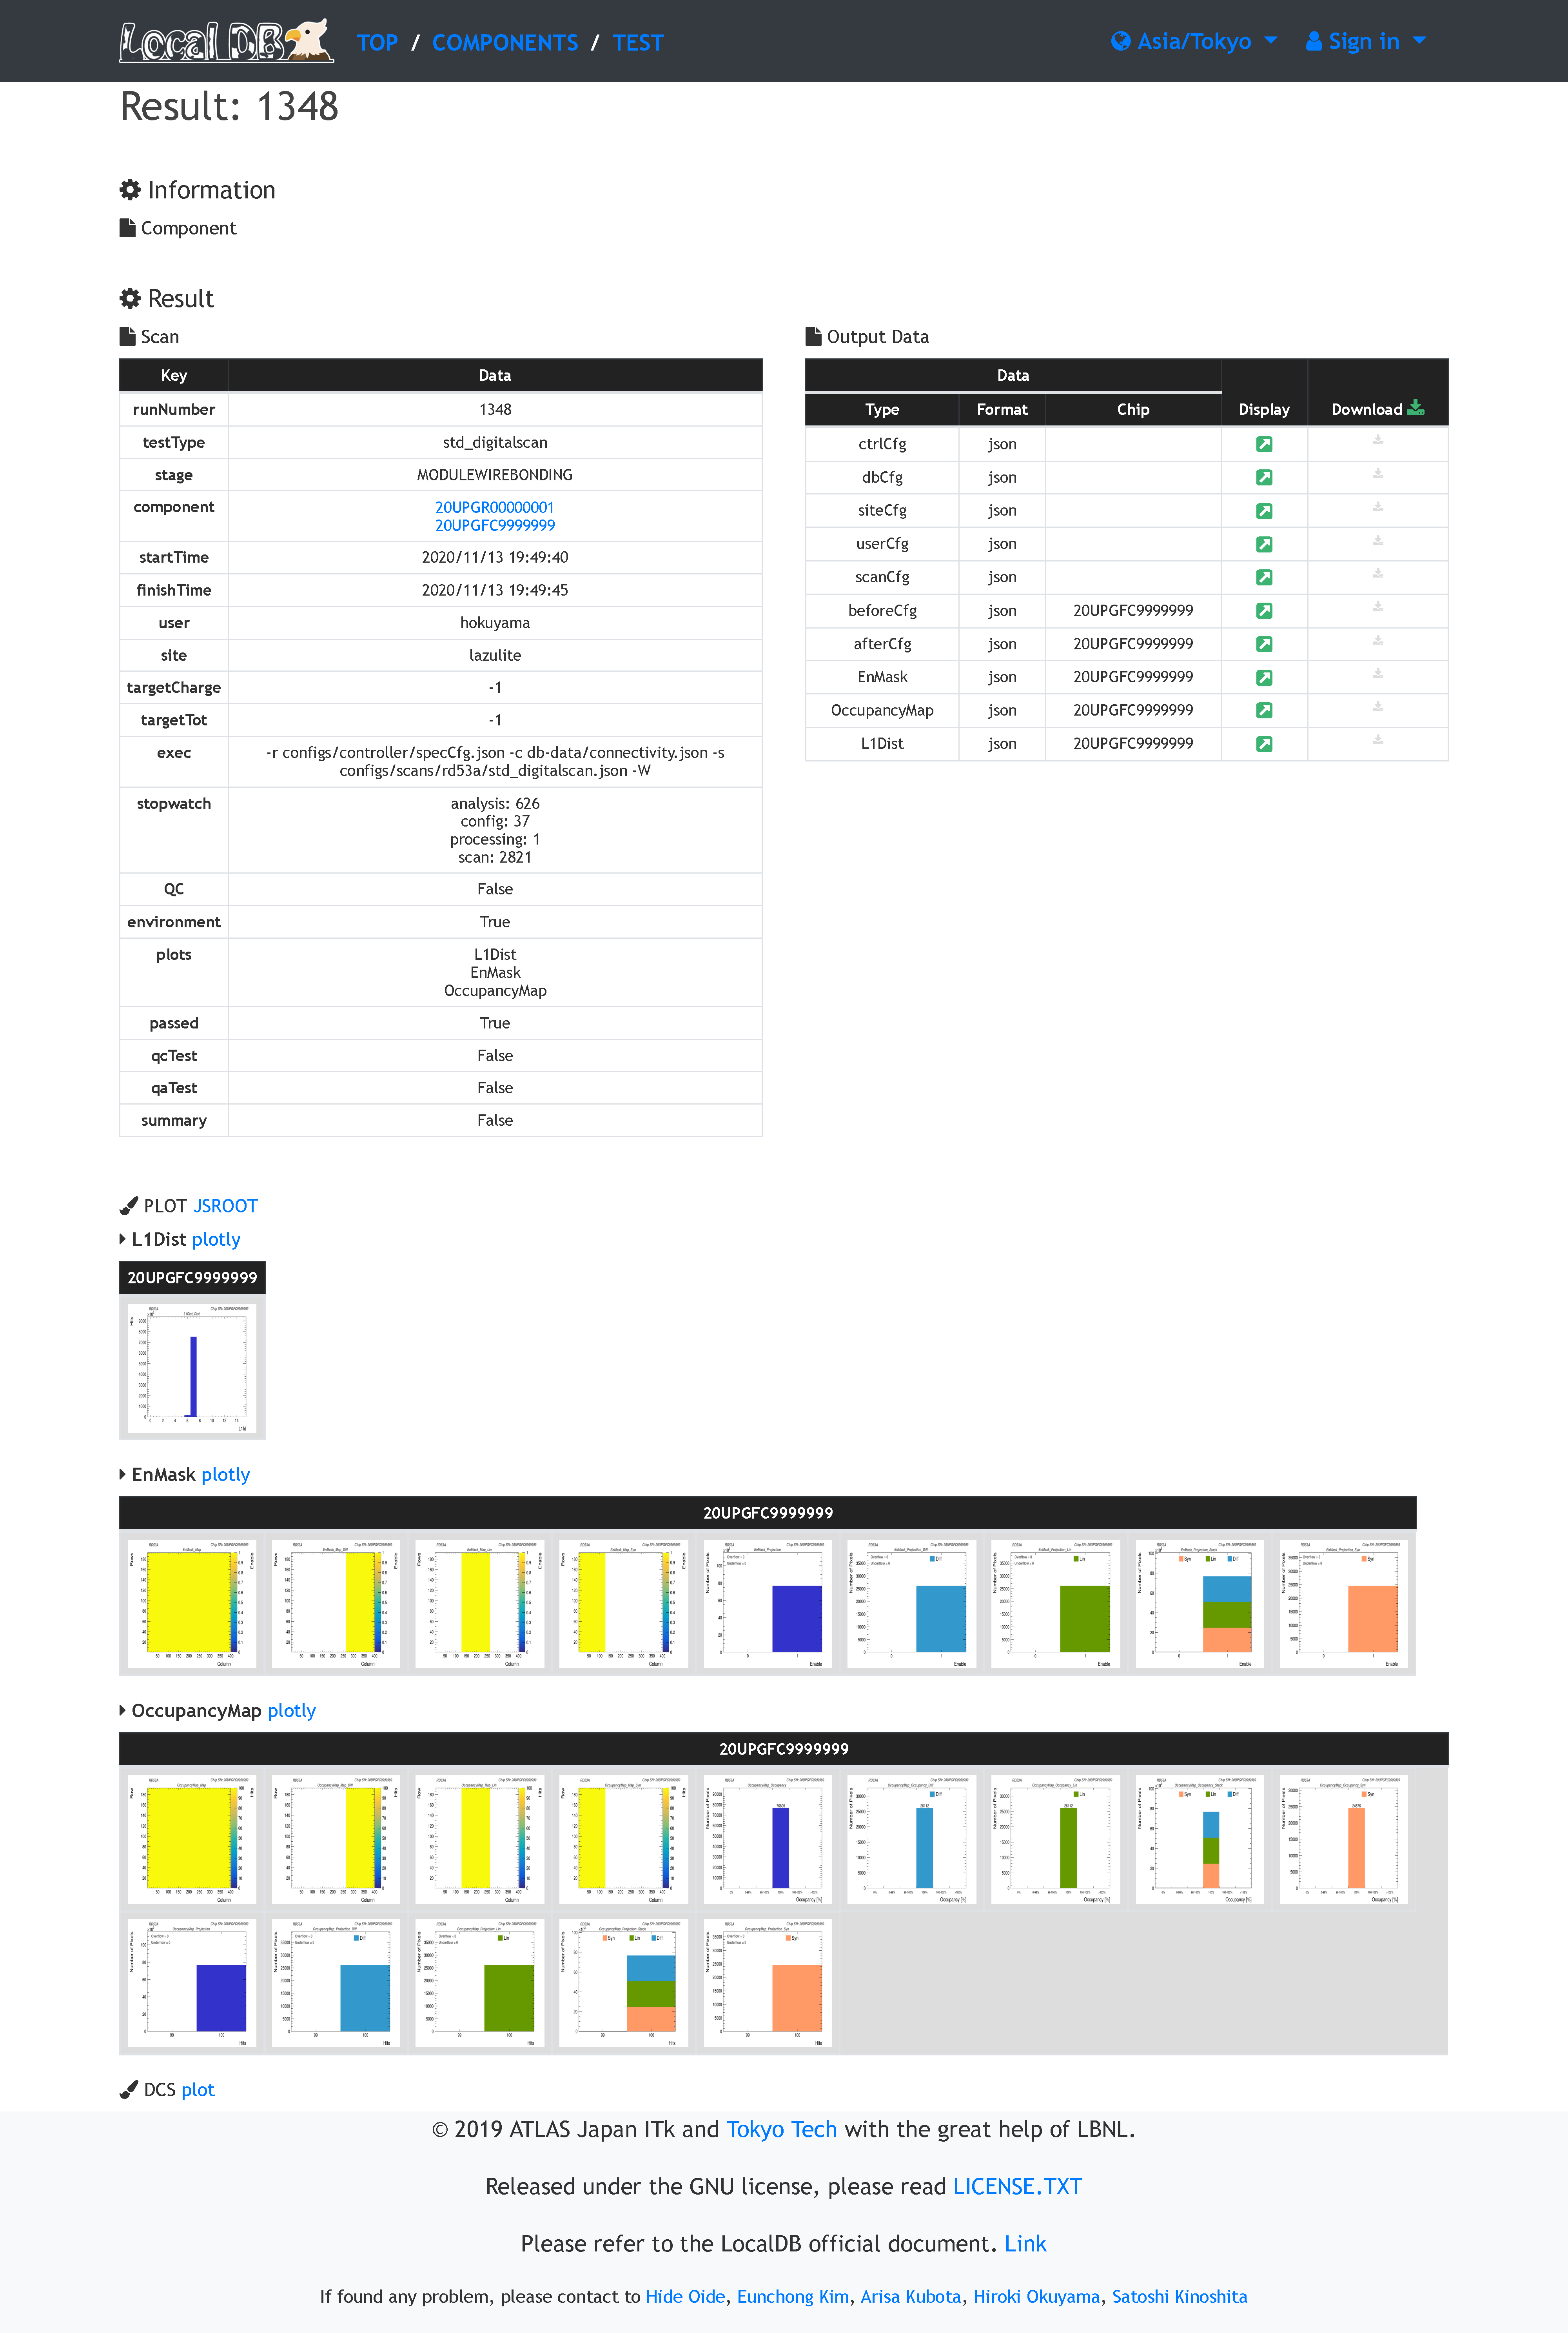
\includegraphics[width=65mm]{demo_view_scan_result.pdf}
    \end{center}
  \end{minipage}
  \begin{minipage}{0.45\hsize}
    \begin{center}
    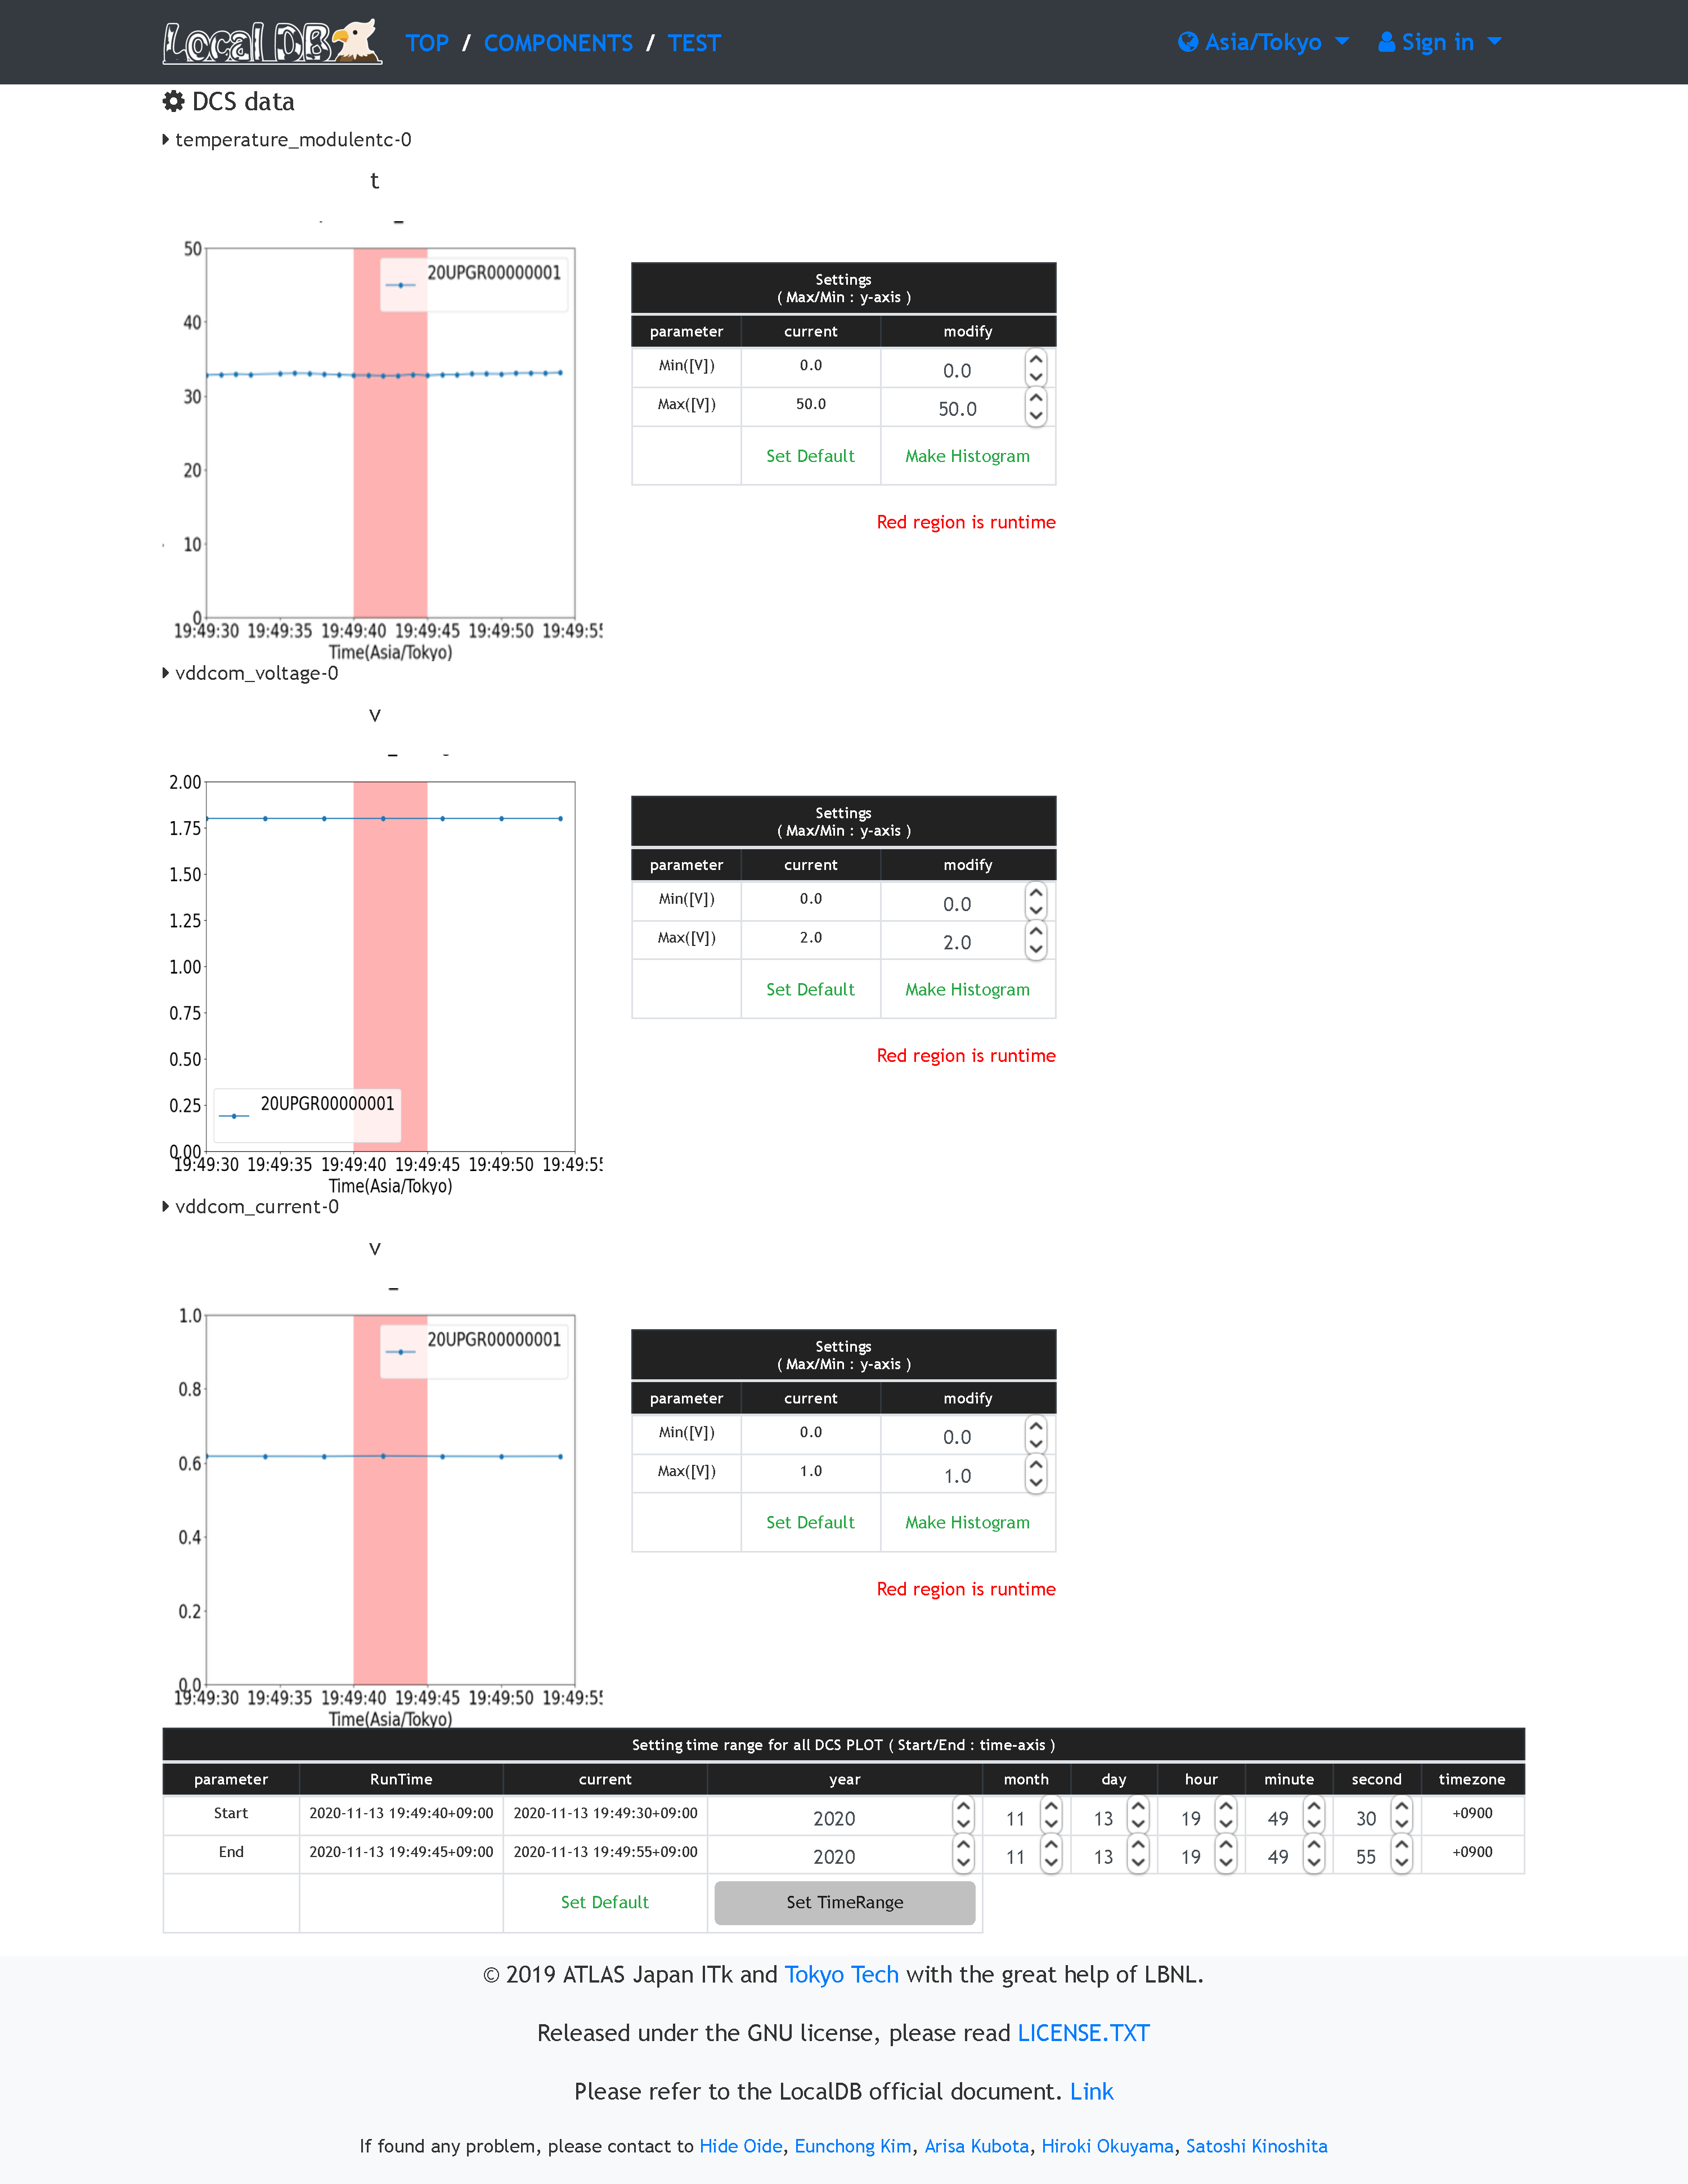
\includegraphics[width=75mm]{demo_view_dcs.pdf}
    \end{center}
  \end{minipage}
  \caption[試験結果の閲覧]{試験結果の閲覧。図は試験結果(左図)と試験におけるDCSデータのグラフ(右図)を示しており、上から温度、電圧、電流となっている。図は\texttt{std$\_$digitalscan}の結果であり、試験情報及び結果のグラフが確認できる。また右図よりDCSデータも正常にローカルデータベース上に保存され、表示されていることが分かる。}
  \label{demo_view_result}
\end{figure}


%%%%%%%%%%%%%%%%%%%%%%%%%%%%%%%%%%%%%%%%%%%%%%%%%
%%%%%%%%%%%%%%%%%%%%%%%%%%%%%%%%%%%%%%%%%%%%%%%%%
\clearpage
\subsubsection{結果選択とピクセル解析}
読み出し結果を選択し、ピクセル解析を行なった。
結果選択画面を図\ref{demo_select_scans}に示す。
このデモンストレーションにおける不良評価基準は3章に述べた表\ref{pixel_analysis_criteria}の中から、現時点でシステムに実装している以下の項目を抜粋した。
\begin{enumerate}
  \item Digital Dead 
  \item Digital Bad 
  \item Analog Dead 
  \item Analog Bad 
  \item Tuning Failed
  \item Tuning Bad for Threshold
  \item Tuning Bad for ToT
  \item High ENC
  \item Noisy
\end{enumerate}

解析結果を図\ref{pixel_analysis_result}、それぞれの評価基準における不良ピクセルの分布を図\ref{pixel_analysis_result_dist}に示す。

\begin{figure}[bpt]\centering
  \begin{center}
    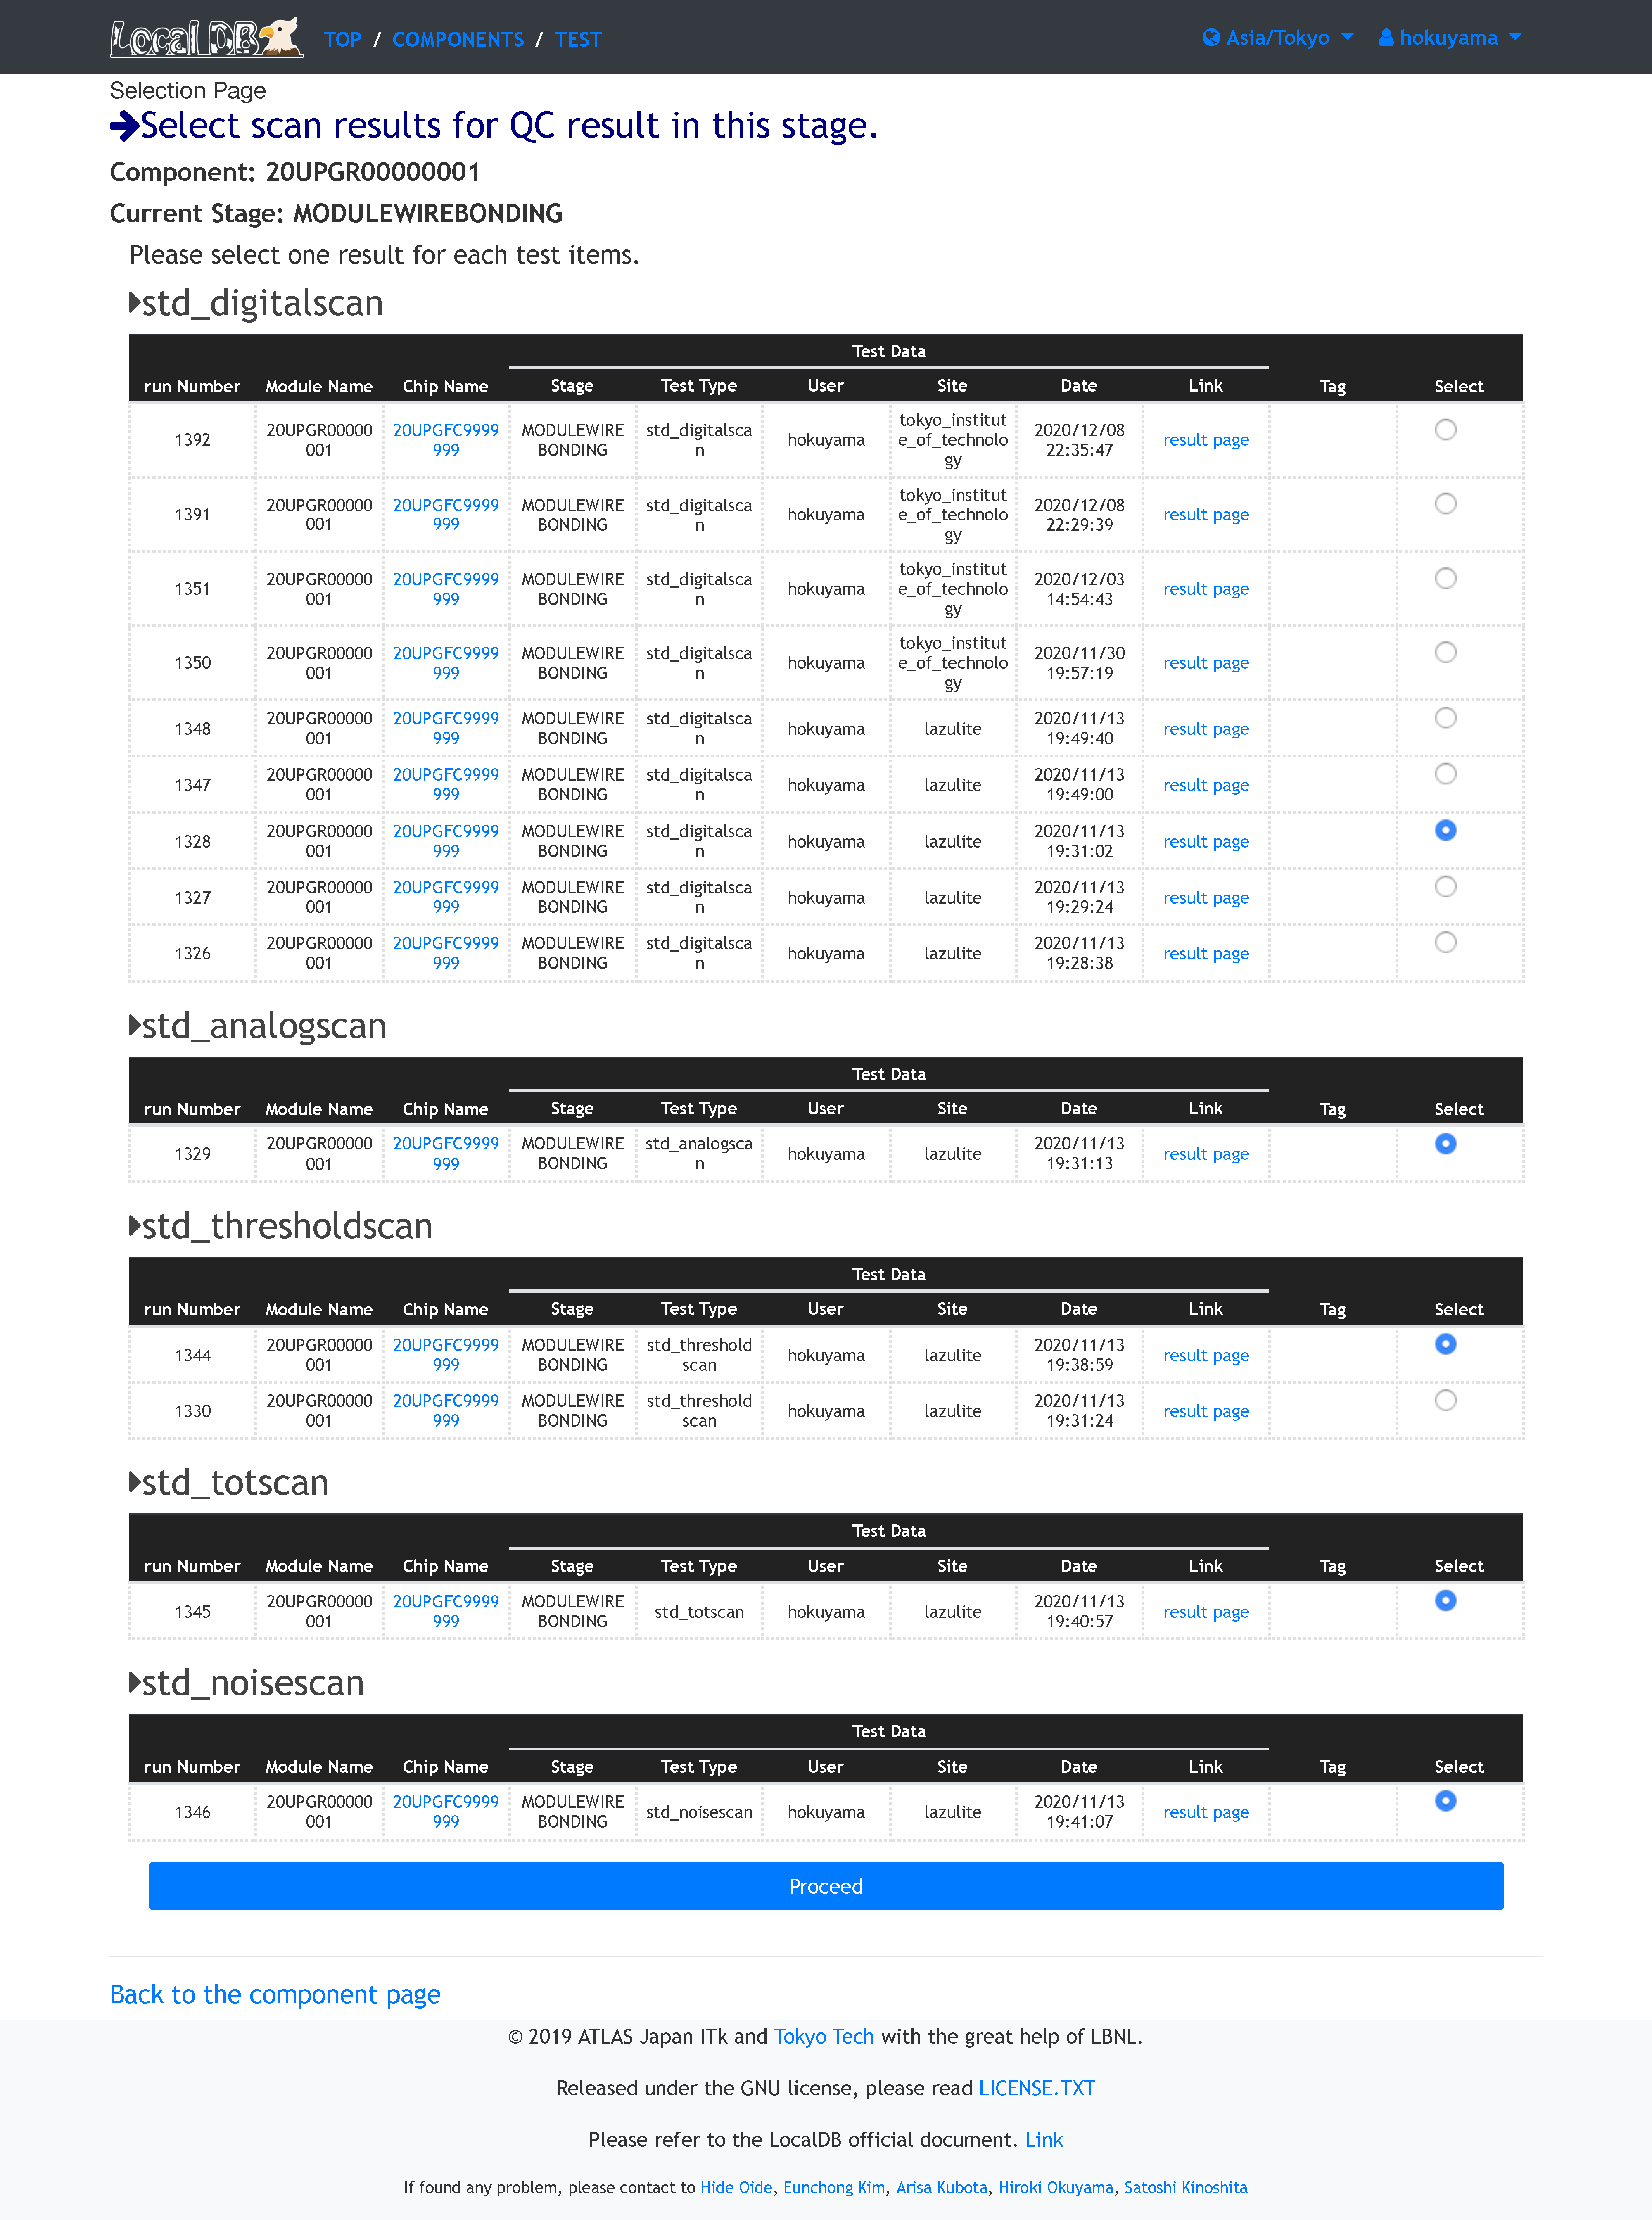
\includegraphics[width=15cm]{./demo_select_scans.pdf}
  \caption[読み出し試験結果の選択]{読み出し試験結果の選択。図は読み出し試験結果選択画面を表す。読み出し試験実施後、ピクセル解析と中央データベースとの同期を実行するために試験結果を選択する必要がある。図では\texttt{std$\_$digitalscan}、\texttt{std$\_$analogscan}、\texttt{std$\_$thresholdscan}、\texttt{std$\_$totscan}、\texttt{std$\_$noisescan}の5項目を選択している。}
  \label{demo_select_scans}
  \end{center}
\end{figure}

\begin{figure}[bpt]\centering
\includegraphics[width=12cm]{./data/analysis_result/Bad_Pixels.png}
\caption[ピクセル解析結果]{ピクセル解析結果。図において横軸は評価基準、縦軸は該当するピクセル数を表す。analog$\_$dead、analog$\_$badの割合が多いため、アナログ回路読み出しに失敗しているピクセルが多いことが読み取れる。}
\label{pixel_analysis_result}
\end{figure}

\begin{figure}[bpt]\centering
  \begin{minipage}{0.45\hsize}
    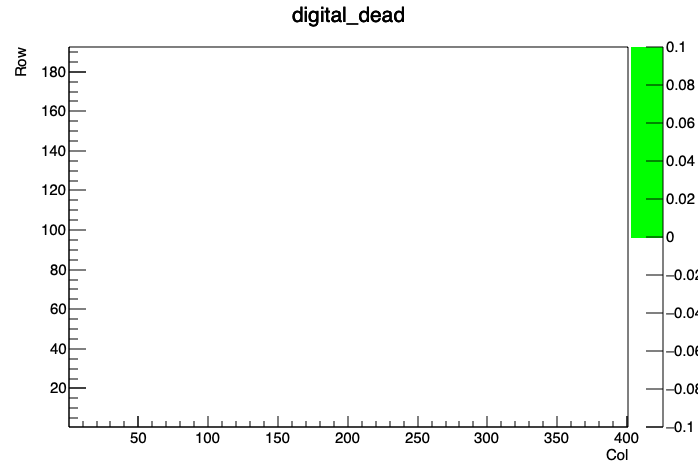
\includegraphics[width=6.0cm]{./data/analysis_result/digital_dead.png}
  \end{minipage}
  \begin{minipage}{0.45\hsize}
    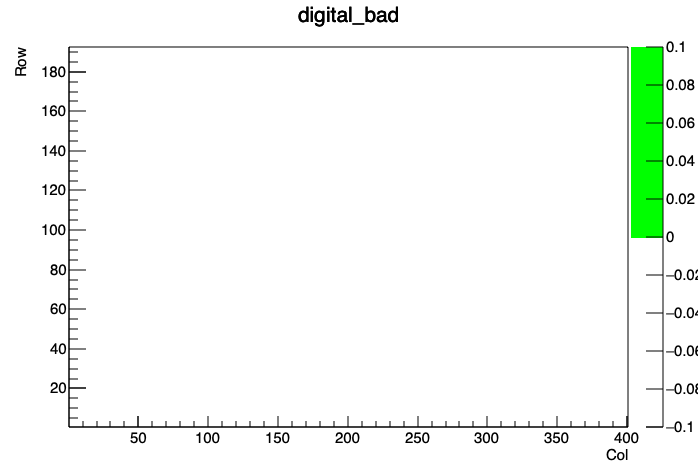
\includegraphics[width=6.0cm]{./data/analysis_result/digital_bad.png}
  \end{minipage}
  \begin{minipage}{0.45\hsize}
    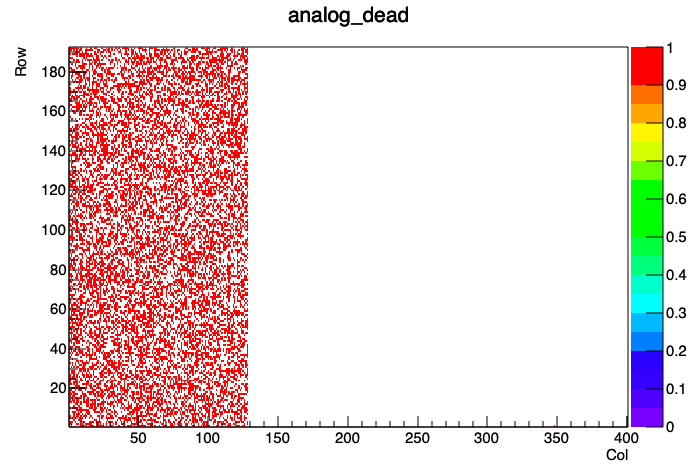
\includegraphics[width=6.0cm]{./data/analysis_result/analog_dead.png}
  \end{minipage}
  \begin{minipage}{0.45\hsize}
    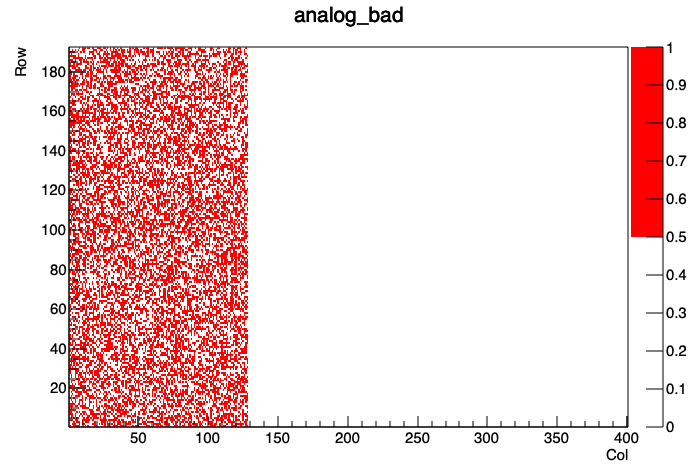
\includegraphics[width=6.0cm]{./data/analysis_result/analog_bad.png}
  \end{minipage}
  \begin{minipage}{0.45\hsize}
    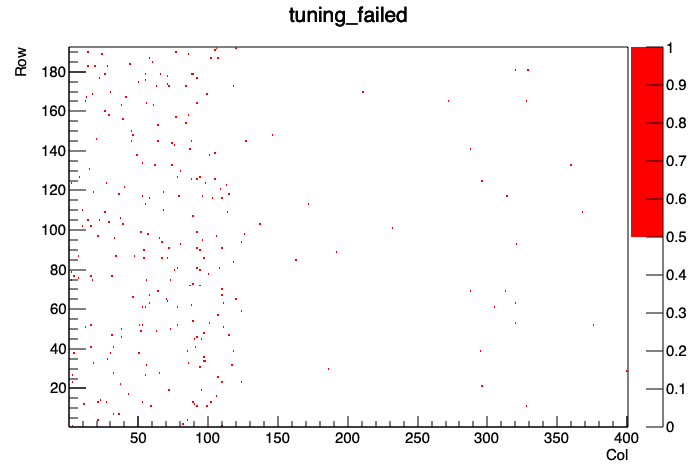
\includegraphics[width=6.0cm]{./data/analysis_result/tuning_failed.png}
  \end{minipage}
  \begin{minipage}{0.45\hsize}
    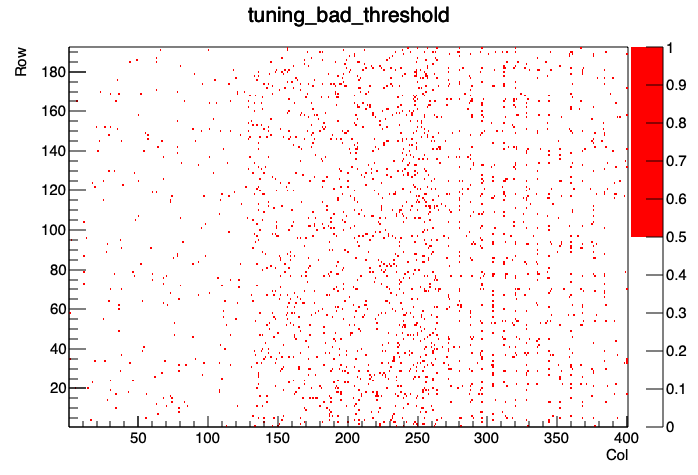
\includegraphics[width=6.0cm]{./data/analysis_result/tuning_bad_threshold.png}
  \end{minipage}
  \begin{minipage}{0.45\hsize}
    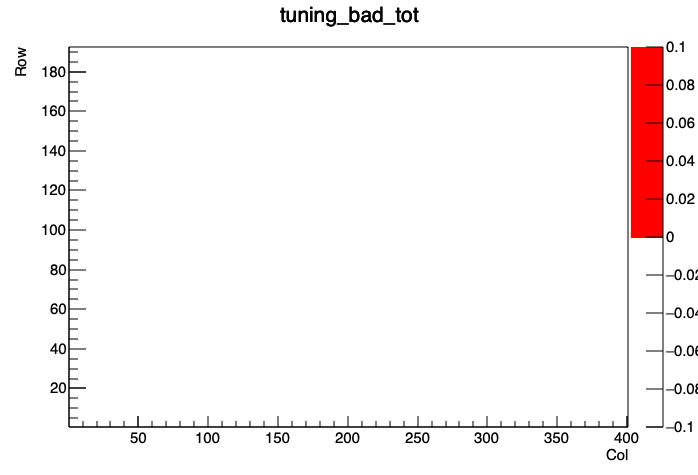
\includegraphics[width=6.0cm]{./data/analysis_result/tuning_bad_tot.png}
  \end{minipage}
  \begin{minipage}{0.45\hsize}
    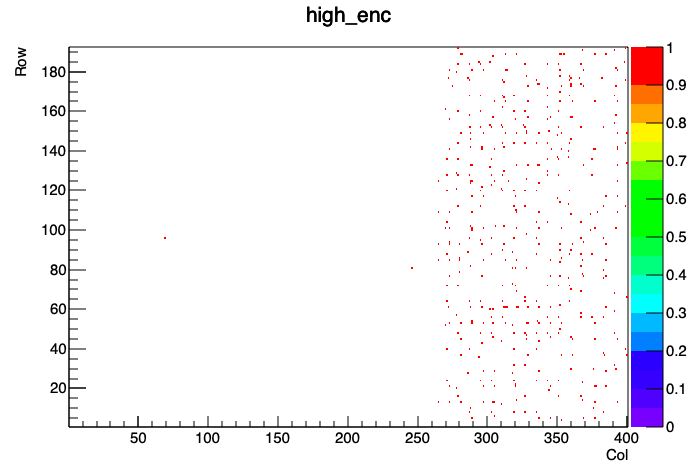
\includegraphics[width=6.0cm]{./data/analysis_result/high_enc.png}
  \end{minipage}
  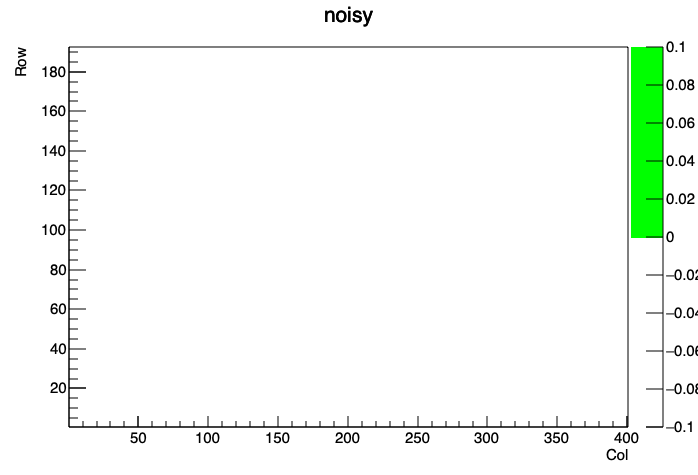
\includegraphics[width=6.0cm]{./data/analysis_result/noisy.png}

\caption[各評価基準における不良ピクセルの分布]{各評価基準における不良ピクセルの分布。各図は二次元ヒストグラムであり、横軸がFEチップにおける各ピクセルの列番号、縦軸が行番号を示しており、赤い領域が不良ピクセルを表している。図\ref{pixel_analysis_result}においてアナログ回路読み出しに失敗しているピクセルが多いことがわかったが、その不良ピクセルはsynchronousフロントエンド上に存在していることが分かる。またThreshold調整に失敗しているピクセル(tuning$\_$bad$\_$threshold)は全体的に分布していることが分かる。}
\label{pixel_analysis_result_dist}
\end{figure}

%%%%%%%%%%%%%%%%%%%%%%%%%%%%%%%%%%%%%%%%%%%%%%%%%
%%%%%%%%%%%%%%%%%%%%%%%%%%%%%%%%%%%%%%%%%%%%%%%%%
\subsubsection{試験結果アップロード}
読み出し試験の結果を中央データベースにアップロードし、情報が正しくアップロードされていることを確認した。
図\ref{demo_upload_to_pd}に中央データベースのウェブページを示す。結果ファイルや解析結果が正しくアップロードされていることが分かる。

\begin{figure}[bpt]\centering
\includegraphics[width=10cm]{./pixel_test_result.pdf}
\caption[中央データベースにおける読み出し試験及びピクセル解析結果画面]{中央データベースにおける読み出し試験及びピクセル解析結果画面。読み出し試験及びピクセル解析結果を中央データベースにアップロードした。図は中央データベースのウェブページを示しており、アップロードされた試験結果画面である。図の中央部に各評価基準における不良ピクセルの数、下部に各試験項目ごとの結果ファイルをまとめたZipファイルが表示されていることが分かる。試験結果のアップロードが正常に完了し、中央データベース上で結果を確認できることが分かる。}
\label{demo_upload_to_pd}
\end{figure}

